% ****** Start of file apssamp.tex ******
%
%   This file is part of the APS files in the REVTeX 4.1 distribution.
%   Version 4.1r of REVTeX, August 2010
%
\documentclass[reprint,%article
 %,
%superscriptaddress,
%groupedaddress,
%unsortedaddress,
%runinaddress,
%frontmatterverbose, 
%preprint,
%showpacs,preprintnumbers,
%nofootinbib,
%nobibnotes,
%bibnotes,
 amsmath,amssymb,
 aps,
%pra,
%prb,
%rmp,
%prstab,
%prstper,
%floatfix,
]{revtex4-1}
\usepackage[table,xcdraw]{xcolor}

%\usepackage{xcolor}

\usepackage{graphicx}% Include figure files
\usepackage{dcolumn}% Align table columns on decimal point
\usepackage{bm}% bold math
\usepackage{appendix}
\usepackage{subcaption}
%\usepackage{subfloat}
%\usepackage{hyperref}% add hypertext capabilities
%\usepackage[mathlines]{lineno}% Enable numbering of text and display math
%\linenumbers\relax % Commence numbering lines

%\usepackage[showframe,%Uncomment any one of the following lines to test 
%%scale=0.7, marginratio={1:1, 2:3}, ignoreall,% default settings
%%text={7in,10in},centering,
%%margin=1.5in,
%%total={6.5in,8.75in}, top=1.2in, left=0.9in, includefoot,
%%height=10in,a5paper,hmargin={3cm,0.8in},
%]{geometry}https://www.overleaf.com/project/5ba0361831a91c7b3990c0d7
 \usepackage{natbib}
 
\begin{document}

\preprint{APS/123-QED}

\title{DRAFT- Rotation Curve Fitting Model }% Force line breaks with \\
%\thanks{ Thanks Jesus}%

% Find out if Joe and Noah still want to be on this paper%

 

\author{Sophia Natalia Cisneros}
 \affiliation{ Department of Astronomy,  
 University of Washington}
 % \email{sophia.cisneros@du.edu}
  \author{Richard Ott}%
 \email{rich.ott@EMAIL.com}
\affiliation{Affiliate MIT - Ask Joe Formaggio}%Tech dudes \textbackslash\textbackslash
%}
 \author{ Meagan Crowley}
\email{ }
\affiliation{NREL}%
 \author{ Amy Roberts}
\email{ }
\affiliation{CU Denver}%
\author{Marcus Paz}
\author{Zaneeyiah Brown}
\author{Landon Joyal}
\author{Roberto Real Rico}
\author{Elizabeth Gutierrez-Gutierrez}
\author{ Phong Pham}
\author{Zac Holland}
\author{Amanda Livingston}
\author{Lily Castrellon}
\author{Shanon Rubin}
\author{Aaron Ashley}
\author{Dillon Battaglia}
%\affiliation{UMass Boston% with \\
%&}%
%
 
 
\date{\today}% It is always \today, today,
             %  but any date may be explicitly specified
             %%%%%%
%%%%%%%
%%%%%%
%%%%%%%
%%%%%%
%%%%%%%
\begin{abstract}
 
 
{\color{teal}   Github repo: Cisneros-Galaxy/RCFM     }

\begin{description}
\item[Usage]
Secondary publications and information retrieval purposes.
\item[PACS numbers]
May be entered using the \verb+\pacs{#1}+ command.
%\item[Structure]
%You may use the \texttt{description} environment to structure your abstract;
%use the optional argument of the \verb+\item+ command to give the category of each item. 
\end{description}
\end{abstract}

\pacs{Valid PACS appear here}% PACS, the Physics and Astronomy
                             % Classification Scheme.
%\keywords{Suggested keywords}%Use showkeys class option if keyword
                              %display desired
\maketitle

%\tableofcontents
%%%%%%NOTES TO DO
%%%make labels for figure axes. remove orange line through the data
%%%%%%
%%%%%%%%
%%%%%%
%%%%%%%
%%%%%%
%%%%%%
\section{Introduction  \label{sec:uno}}


%DARK MATTER

 The flat-rotation curve problem of spiral galaxies  is viewed as primary evidence for dark matter\cite{Rub,Bosma,1985ApJAlbada}. 
 The dark matter paradigm interprets the divergence of two kinematic phrasings of         observations of light, spectra and photometry (see Fig.~\ref{fig:NGC2403}),     as a missing mass component. 
 Photometry yields Keplerian orbital velocities, which fall-off outside of the stellar light. Doppler shifted spectra yields rotation velocities from the Lorentz Doppler shift formula, which do not fall-off outside the stars.  
 Dark matter theories are built from classical gravity,   with massive
   ``dark'' particles  which do not interact electromagnetically.   These particles have   yet to be    discovered, but are hypothesized to have a very low interaction probability with baryonic matter, and so  experiments are ever increasing   sensitivity to detect them \cite{Cebrian:2022brv}. In the absence of a direct detection, the paradoxes of dark matter models are interesting. 
   
   The first paradox is best stated by 
  S. McGaugh  when they ask   ``Why is the luminous tail wagging the dark matter dog,  if dark matter dominates dynamics ?'' \cite{1999McGaugh,McGaugh2016RAR}. This is known as the  disk-halo conspiracy, and references the strange fact that knowledge  of 
 the luminous stellar   disk  completely determine the spherical dark matter halo \cite{2004ApJ...609..652M}.  
 
 
 
 A second paradox  is known as  the Universal Rotation Curve(URC)  \cite{salucci,Persic,1978Rubin,10.1111/j.1365-2966.2007.11696.x}, in which  a spectrum of 1,100 galaxy rotation curves
 inflect  about  the Milky Way's    (Fig.~\ref{fig:URC}).  This spectrum requires   
  small less dense  dwarf galaxies to have accreted   proportionally larger dark matter halos than   huge, centrally dense    galaxies. 
   In dark  matter models this result requires fine-tuning, since
  classically mass accretion rates are proportional to total mass \cite{10.1093/mnras/stt2403}.  
  This reduces the model's    predictivity   \cite{MCGAUGH2021220}. 
  
  
  We will   interpret these paradoxes   as  indicative of  frame-dependent effects,   due to the Milky Way. 
   Previously, the role of relative
     galaxy curvature  in this problem  were    obviated 
       by  Galilean subtraction of   gravitational red-shifts at the  large $r$  limit of the data \citep{MTW}. 
     The leading   alternative    to dark matter theory  in the flat-rotation curve problem is   Modified Newtonian Dynamics (MOND) \cite{Milgrom}.  MOND    proposes    
     a changing  physical law of gravity,    on the vast distance scales of galaxies, and  that the   luminous mass is the only mass   \cite{McGaugh_2014}. 
  This approach  is   predictive across a  broad  sample of galaxy rotation curves,  representing diverse    sizes and morphologies \cite{2016Lelli}.  MOND uses only   a single, roughly constant free-parameter to represent the new acceleration scale for all spiral   galaxies  \cite{McGaugh2016RAR,2022A&A...664A..40M}, although there are a few interesting galaxies where the MOND prescription requires galaxies to be at different distances than indicated by Cepheids/SN(CITE) . 
  
  
  Previous extensions of MOND into the relativistic regime have given rise to  new theories of gravity  \cite{PhysRevD.70.083509,doi:10.1142/S0217751X0703666X,Famaey2012}, but we present   a more economical interpretation of   MOND's changing acceleration   transitioned to  the relativistic concept  of  changing   relative curvatures.   
  In this paper we   introduce a new  technique for  transformations     between galaxies,  to replace dark matter, and demonstrate the success of this approach by developing the fitting formalism and fitting   a sample of 174 galaxy rotation curves previously fitted by the MOND and dark matter models  \cite{McGaugh2016RAR,2016Lelli,McGaugh_2014,Li_2018}.  
       At this time, there are many problems in   the concordance model of   cosmology which are attributed to dark matter \cite{2010dmp..book.....S,Tully:2014gfa,Naidu_2022}, but in
 this paper we address only this  one. 
    Modeling of 
dark matter halos remains severely   under-constrained with correlated parameters including radius, slope, scale length, and halo core radius (CITE).     
The technique presented here, whether fundamental or no,  has the advantage of replacing the dark matter term  with a product of terms based only on estimates of the luminous mass and   a single free parameter.
   
      
  
 
 
 
This paper  is organized as follows;
{\bf Section \ref{sec:dos}} constructs  the rotation curve  fitting formula, 
{\bf Section \ref{sec:data}}   describes  the data we use, 
 {\bf Section \ref{sec:analysis}}   discusses our results, 
 and  {\bf Section \ref{sec:conclu}}   discusses implications for future tests.   
  
  
 \begin{figure}[h!]
     \centering
     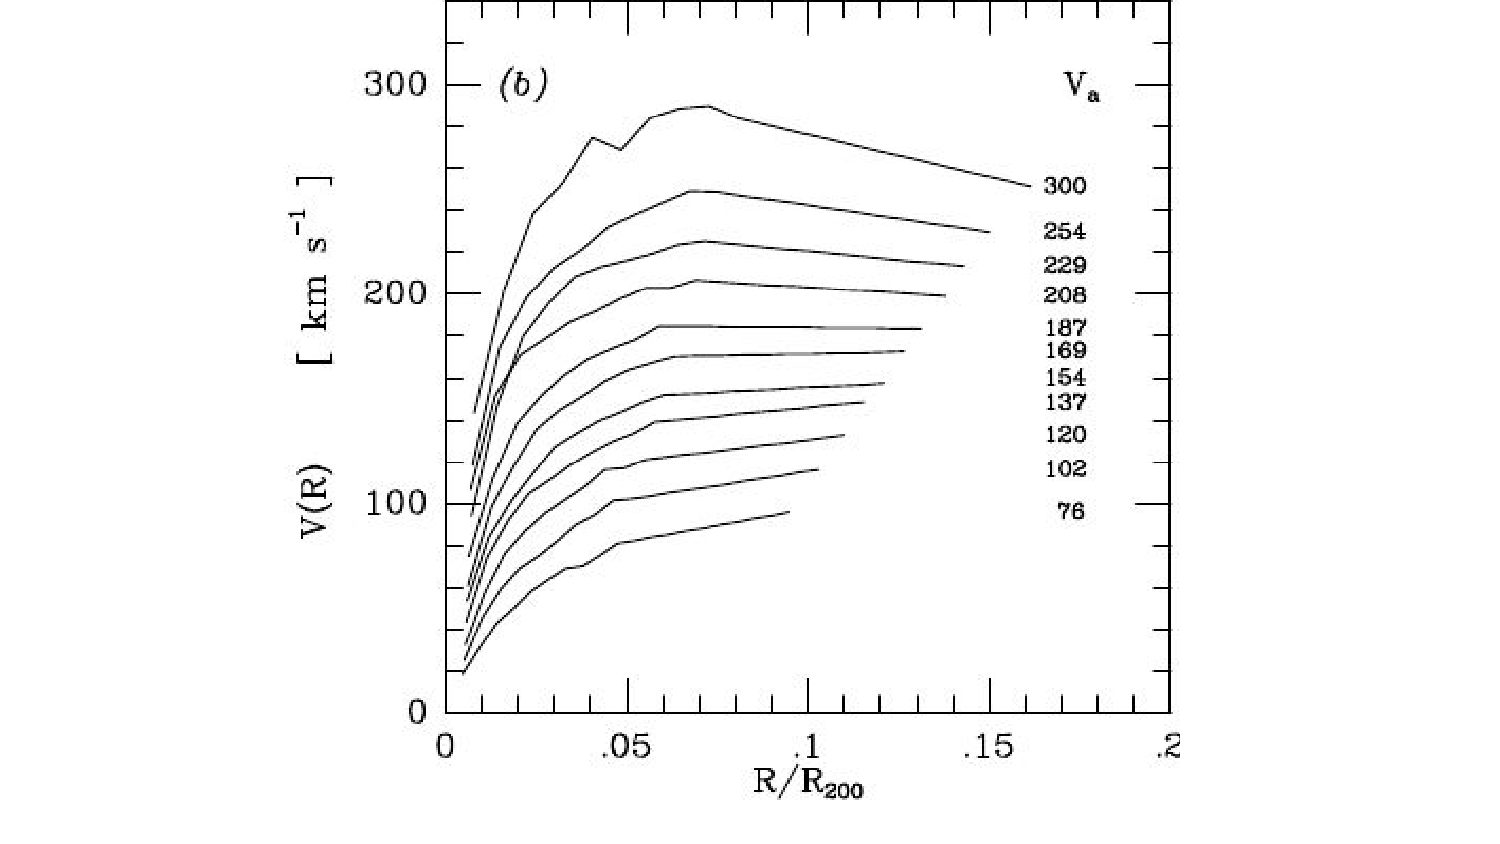
\includegraphics[width=\linewidth]{URC}
     \caption{\emph{Universal Rotation Curve spectrum, Used with permission from Ref.\citep{salucci}}}
     \label{fig:URC}
\end{figure}
  

  
    
 \begin{figure}[h!]
%\scalebox{0.25075}%
      \centering
      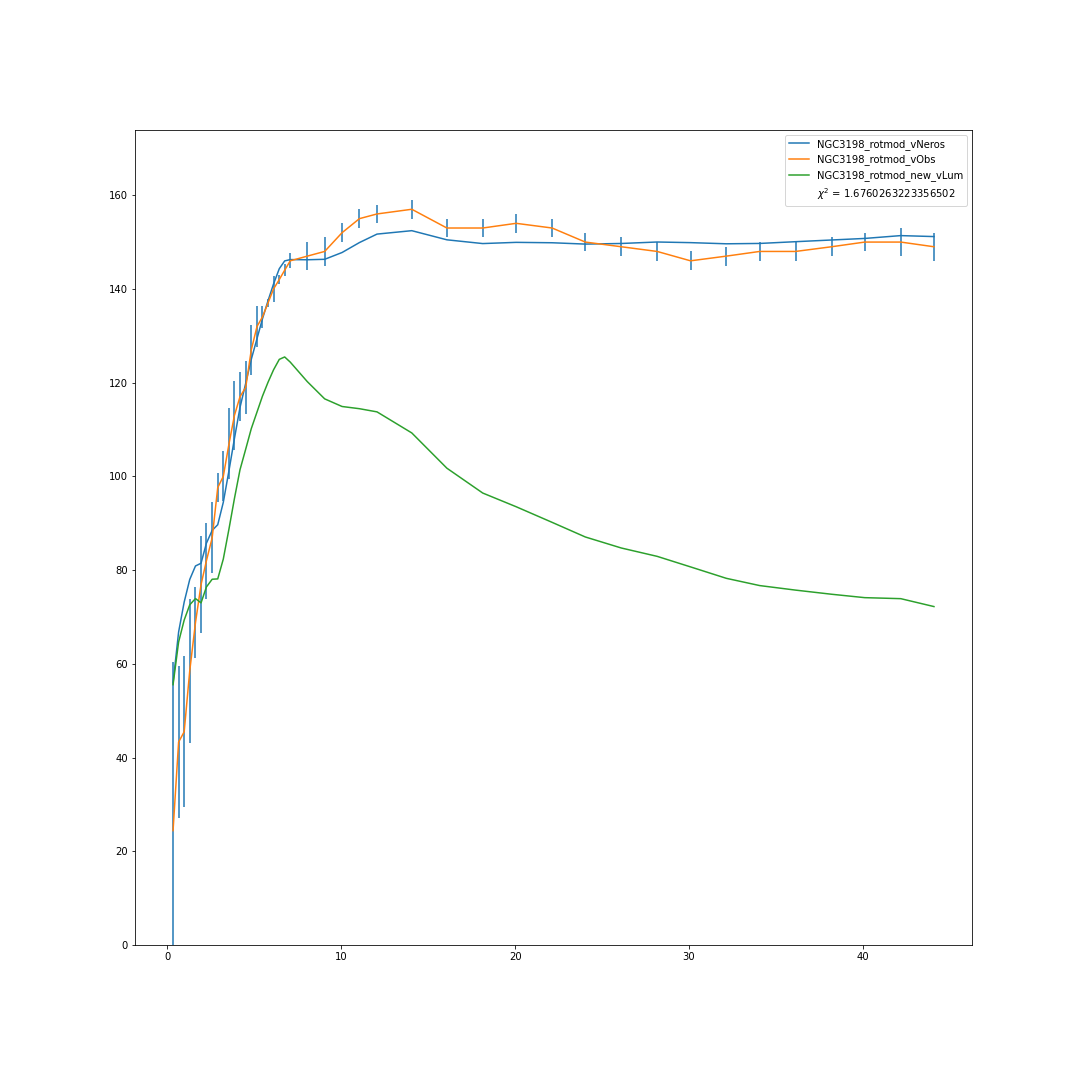
\includegraphics[width=\linewidth]{figures/NGC3198_rotmod_XueSofue.png}
      \caption{\emph{Rotation Curve of NGC 2403 \cite{Blok1}.   Rotation curve data blue dots with  error bars,  Keplerian velocity from luminous mass estimated by   green line,   RCFM fit blue line.} }
      \label{fig:NGC2403}
  \end{figure}
%%%%%%
%%%%%%%%
%%%%%%
%%%%%%%
%%%%%%
%%%%%%
\section{Rotation Curve Fitting Formulae  \label{sec:dos}}
 
 
 \subsection{Dark matter rotation curve fitting formula}
 
  

 The   dark matter rotation curve formula   is of the form

 \begin{equation}
v(r)^2_{obs}  =  v(r)^2_{lum}  +  v(r)^2_{dm},   
\label{eq:zonte1}
\end{equation} 

  where all velocities are assumed to be circular orbits, in the plane of the disk,  about the rotation axis of the galaxy at  $r=0$. 
Terms in  $v_{obs}$ are the velocity parameters   of a  Lorentz boost
   

 \begin{equation}
 \frac{v_{obs} }{c}=
\frac{  \left( \frac{\omega'(r)}{\omega_o}\right)^2 -  \left( \frac{\omega_o}{\omega'(r)} \right)^2 }{  \left( \frac{\omega'(r)}{\omega_o}\right)^2  +  \left( \frac{\omega_o}{\omega'(r)}\right)^2 },
\label{eq:modelLumA}
\end{equation} 

 in flat Minkowski spacetime. The    
  characteristic rest-frame frequency is $\omega_o$, the  observed  Doppler shifted frequency is $\omega'$, and $c$ is the constant vacuum light speed.  
 Terms in  $v_{lum}$ are from observations of total light  (photometry) interpreted by Population Synthesis Models (PSM) mass-to-light ratios as mass,   hence orbital velocities  
  
   \begin{equation}
v(r)_{lum}^2 = \gamma_b v(r)_{bulge}^2 +  \gamma_d v(r)_{disk}^2 + v(r)_{gas}^2.    
\label{eq:zonte3}
\end{equation} 
  
 Terms in    $\gamma_i$  are the mass-to-light ratios for the stellar bulge $\gamma_b$ and disk $\gamma_d$ respectively, which come from PSM. Gas measurements do not require  a mass-to-light ratio due to different measurement techniques(CITE).  
 Terms in $v^2_{dm}$ represent
the dark matter, which is  the algebraic difference of the   terms  $v^2_{obs}-v^2_{lum}$. 

    Eq.~\ref{eq:zonte1} and Eq.~\ref{eq:zonte3} are quadratic    sums to represent  sums of the  gradients in the potential,  as a function of  radius, 
 for each mass contribution to the  central gravitational    force law   

\begin{equation}
 \frac{\partial \Phi(r)_{lum}}{\partial r}    =\frac{v(r)_{lum}^2}{r},  
    \label{zoochance1}
\end{equation}

  
   
where the   Newtonian gravitational potential is

\begin{equation}
      \Phi(r)  = -G \int d^3r'  \frac{ \rho(r') }{r-r'} ,
      \label{eq:Newt}
      \end{equation}

which solves Poisson's equation

\begin{equation}
\nabla^2 \Phi(r)_{lum}  = 4\pi G \rho(r)   
    \label{whatsgood}
\end{equation}

 for $G$  Newton's   gravitation constant, and 
$\rho(r')$  the mass density. 
  



\subsection{New Rotation Curve Fitting Formula}

  

 

 To test the   new 
frame-dependence picture, 
we  replace the gradient in the potential   attributed to   dark matter      with  Lorentz-type transformations between galaxy frames.   We    assume  luminosity   is a Lorentz scalar, therefore invariant under the assumption of a good distance estimate, and   a faithful tracer of baryonic mass.  We assume baryonic mass is the only mass in this problem. 
We assume   
   Doppler shifted spectra is part of a Lorentz 4-vector, and so    must transform in a Lorentzian sense.
In addition, we 
   assume   shifts in   spectra   due to relative velocity and relative acceleration are separable \cite{Jack,Cisn}, perhaps roughly  as in Eq.~\ref{eq:zonte1}.
  In what follows, all   terms  can be assumed to  be functions of radius except the model's free parameter $\alpha$,  which is single valued for each galaxy fitted and the speed of light $c$. 
   
   The new rotation curve formula we propose  is
   

\begin{equation}
v_{rc}^2 =  v_{lum}^2+\alpha \kappa^2 v_{1} v_{2},  
\label{eq:zonteLCM}
\end{equation}  

for $\alpha$  a free parameter,  
$\kappa$  a curvature ratio 

 \begin{equation}
\kappa=\frac{\Phi_{gal}}{\Phi_{mw}}, 
\label{eq:kappa2}  
\end{equation}  

 and $\Phi_{gal}$ the    Newtonian gravitational potential of the galaxy being observed, and $\Phi_{mw}$ that of  the Milky Way, one-to-one in radii. 


 Terms in $v_1$   are   
 
   \begin{equation}
       v_1 = \sinh \zeta. 
   \end{equation}
 
 for a rapidity angle $\zeta$ defined by the    Lorentz exponential  term  
  
   
     \begin{equation}
     e^{\zeta}=  \frac{\omega_{mw}}{\omega_{gal}}  =\sqrt{\frac{g_{tt}|_{gal}}{g_{tt}|_{mw}}},
      \label{eq:gravRS}
    \end{equation}
    
 for  clock terms $g_{tt}$   defined in the   weak field Schwarzschild limit  \cite{Hartle}, 
 
  \begin{equation}
      g_{tt}= -( 1 - 2\Phi/ c^2).
      \label{clocktime}
  \end{equation} 
  

Terms in $v_2$ are 

\begin{equation}
v_{2} =  \cosh \tau, 
\label{eq:hyperbolico}
\end{equation}


 
 
  for a rapidity angle $\tau$ defined by the    Lorentz exponential  term  
  
 
\begin{equation}
    e^{\tau}=   e^{(\zeta+\eta)/2},
\end{equation}
 
for the  flat field-frame
Lorentz exponential  

\begin{equation}
    e^{\eta}=\frac{\omega_{l}}{\omega_o}= \sqrt{\frac{1+\beta}{1-\beta}}.   
    \label{eq:flat}
\end{equation}  
     
Terms in 
$\beta = v_{lum}/c$ are the
Keplerian rotation velocities  estimated from total light  $v_{lum}$, and  associated with  frequency shifts $\omega_{l}$      by a Lorentz boost   

 \begin{equation}
 \frac{v_{lum} }{c}=
\frac{  \left( \frac{\omega_{l}}{\omega_o}\right)^2 -  \left( \frac{\omega_o}{\omega_{l}} \right)^2 }{  \left( \frac{\omega_{l}}{\omega_o}\right)^2  +  \left( \frac{\omega_o}{\omega_{l}}\right)^2 }. 
\label{eq:lumlorentz}
\end{equation} 
 
 
  
 
 
The   term $v_1$ maps the gravitational frame of the observed galaxy into that of the Milky Way. The   term $v_2$    maps from  the   curved 2-frame  of  Eq.~\ref{eq:gravRS},  to  the flat 2-frame where we make observations. 
  That this second transformation  is necessary is evidenced by the local constancy of the speed of light. 
  We assert that Keplerian rotation curves are     the best estimate of flatness, since dark matter is not required to  reproduce the rotation curve of our Solar System.
 
    
  
 
  A heuristic construction  and assumptions for integration of the gravitational potentials are described in the next section. Fitting details and analysis are reported in Sec.~\ref{sec:analysis}. 
   
 

 
 
%%%%%%
%%%%%%%
%%%%%%
%%%%%%%  
%%%%%%
%%%%%%%  
\subsection{Gravity Details \label{sec:gravDets}}

 
    The relative galaxy transformations in   Eq.~\ref{eq:zonteLCM}, $v_1$ and $v_2$,  are
    constructed in  the following heuristic way.  
Lorentz exponential terms (Eq.~\ref{eq:gravRS} and Eq.~\ref{eq:flat})
  are    identified  as the field frame relationships defining the $v_1$ and $v_2$ transformations. We arrive at this result  by  comparison of 
     the  Lorentz transformation in  Eq.~\ref{eq:modelLumA} with 
 that of the    hyperbolic form \cite{rindler2013essential} 


     \begin{equation}
         \frac{v}{c} = \tanh \theta = \frac{e^\theta - e^{-\theta}}{e^\theta + e^{-\theta}} .   
         \label{boost}
     \end{equation} 

 The  $v_1$ and $v_2$ functions reported here have been   selected based on goodness of fit, for tests of various hyperbolic functions  explored in   \cite{Cisneros:2013vha,Cisneros:2014fea,Cisneros2015,Cisn2016}. 
 The  $v_1$ and $v_2$  functions 
 reported here fit the galaxies in the SPARC sample twice as well as the previous functions fit the same sample. 
 Note, when viewed as    Rindler's accelerated coordinates\cite{MTW,Wald, rindler2013essential}, the   $v_1$ term is  timelike   and $v_2$ is spacelike. 
 
 
 
Lorentz exponential terms in  $v_1$ and $v_2$ are parametrized with ratios of  the    Schwarzschild gravitational redshifts

\begin{equation}
       \frac{\omega_1}{\omega_2}  =\sqrt{\frac{g_{tt}|_{P2}}{g_{tt}|_{P1}}} =\sqrt{\frac{|\xi^t\xi_{t}|_{P2}}{|\xi^t\xi_{t}|_{P1}}}.
      \label{eq:grav}
    \end{equation} 
    
    This formula is    intended to represent the changes in a photon frequency moving from point $P1$ to $P2$, for both points in the same manifold. 
To extend the relationship Eq.~\ref{eq:grav} to connect 
  two distinct gravitational manifolds,   we note that Eq.~\ref{eq:grav} came from  the conservation properties of  the timelike  Killing vector fields  
   $\xi^t(r)$  \cite{Wald}.   The timelike Killing fields rely on  the
  $g_{tt}$, 
  which   rely on the Newtonian  gravitational potentials about the galaxy center Eq.~\ref{eq:grav}. 
  To relate two galaxies, then, is to consider the  potentials. 
  
  
   Wolfgang Rindler said,        ``the center of each galaxy provides a basic local standard of nonacceleration ... so then can be treated like a local inertial frame relative to its own center.''\cite{rindler2013essential}.
 In a globally flat spacetime, $\Phi$ is integrated from the outside to the inside, from a value of  zero potential at the large  $r \to \infty$ limit, into a negative maxima at   $r\approx 0$. 
This procedure  ensures   energy goes to zero at infinity.  However, 
  the external environments of galaxies at the large $r$  limit of the data are extremely complicated  and diverse \cite{Pomarede:2020pme,Hoffman:2017ako}, and cannot be compared to zero in any meaningful way.
    We do know a place where the behavior of the $g_{tt}$ are all equivalent, where     clocks all read the same   $t=0$, at the event horizon of the central  galactic black hole. 
 
 
   
   
 To insure that all galaxies are compared from the same zero, we reverse the order of integration,   

 \begin{equation}
    | \Phi | = \left|  \int^{R-big}_{r-small} \vec{F_r}\cdot\vec{dr}\right|.
      \label{eq:Newt2}
      \end{equation}
 
 

   We posit that this allows all galaxies to be  compared as Rindler's inertial frames, and then that Lorentz boosts can be accomplished in $g_{tt}$.
 Potentials calculated in this way still obey the central force law for test particles moving in circular orbits in Eq.~\ref{zoochance1} and Poisson's equation Eq.~\ref{whatsgood}.
   
 

%%%%%%
%%%%%%%
%%%%%%
%%%%%%%
 
 %We   assume   the  additional symmetry of the  Tetrad-formalism \cite{BertschingerClassTetrads}, which attaches  a    local Lorentz frame   at each point in the manifold 
   % \begin{equation}
      %  g^{\mu \nu} = \eta^{\alpha \beta} e^\mu_\alpha  e^\nu_\beta
   % \end{equation} 
    
  %  so that the orthonormal  basis vectors  $e^\mu_\alpha$ carry the information of the physical spacetime, and the tetrad at each point is Lorentzian and   can endure 3 boosts and 3 rotations \cite{BertschingerClassTetrads}.  
% 
%-  WALD - the basis is the $e^\mu$ and these are $\sqrt{g_{tt}}$ so they not flat, but inner product of one of those bad boys with the inverse covector of the other galaxy, would give us eq. 10, also checkiyo if the indices are correct, originally had a, b lower indices on the basis. CHECK) 
%%%%%%
%%%%%%
%%%%%%% 
%%%%%%
%%%%%%
%%%%%%%  
%%%%%%
%%%%%%%  
%%%%%%
%%%%%%%
\section{Data \label{sec:data}}
 
 \subsection{SPARC }
 We fit the SPARC dataset  of  175 nearby galaxies with extended rotation curves from atomic hydrogen (HI)  and H-$\alpha$ (Spitzer Photometry and Accurate Rotation Curves)\cite{2016Lelli}. HI provides the most reliable
 rotation curves because it dynamically cold, traces circular orbits, and can be observed several effective radii past the stellar disk. This sample of rotationally supported galaxies   spans the widest range of masses and morphologies currently available. In addition, these galaxies are  accompanied by luminous mass models which come from   Spitzer Photometry in the 
   near infrared  at 3.5$\mu m$, which is widely believed to be the best tracer of stellar mass   in population synthesis models and   gives mass-to-light (M/L) ratios which are almost constant, independent of star formation history \cite{BelldYong,10.1093/mnras/sty3223}.  Stellar M/L ratios   translate   photometry to dynamics. 
   
   
     All terms in $\Phi(r)$ used in this paper  are    integrated from estimates of the baryonic mass, reported kinematically as in Eq.~\ref{eq:zonte3} in the      SPARC  library.   These velocities  are constructed from photometric observations of surface brightnesses, interpreted   by a Population Synthesis Model (PSM)\cite{10.1093/mnras/sty3223} as     masses. 
PSM rely upon a complex  suite of  assumptions regarding galaxy evolution, metallicities and initial mass functions  \cite{BelldYong,10.1093/mnras/sty3223}. PSM predict   mass-to-light ratios  $\gamma_i$
 which translate  luminosity into mass dynamics as in Eq.~\ref{eq:zonte3}. 
     The $v_{disk}$ and $v_{bulge}$ are reported in the SPARC database with $ M/L = 1$ in units of  $M_{\odot} / L_{\odot}$   at 3.5$\mu m$.
     Gas fractions $v_{gas}$ are calculated from surface density profiles of HI  with the formalism given in  \cite{1983MNRAS.203..735C} and scaled 
     a factor 1.33 to account for cosmological helium abundances.  
     Contributions from molecular gas are ignored   because CO data are not available for most SPARC galaxies. 
     Error on these velocities is estimated at $20\%$ \cite{2016Lelli}. 
     
      
  
 

  
%ASK STACY: they use M/L =1, so why he say mines are high? 
   %but also says in Lelli 2016 paper they use 0.5\gamma for M/L
 %Their final science sample is made of 153 galaxies.
 


%%%%%%
%%%%%%
%%%%%%%
\subsection{Milky Way}
%''Mapping the Milky Way is one of the key science drivers for LSST.''~Mario Juric ,  UW
The rotation curve fitting model presented here requires a static choice for the baryon distribution of the   Milky Way (MW).   This is an under-constrained problem, due to  the    problem of observing from       inside  the system  \cite{1991ARA&A..29..409F}.
 Outside of our position at 8 kpc in the disk of the MW, the data is very 
 noisy, see  Fig.~\ref{fig:mwSofue}.
 
 \begin{figure}
    \centering
    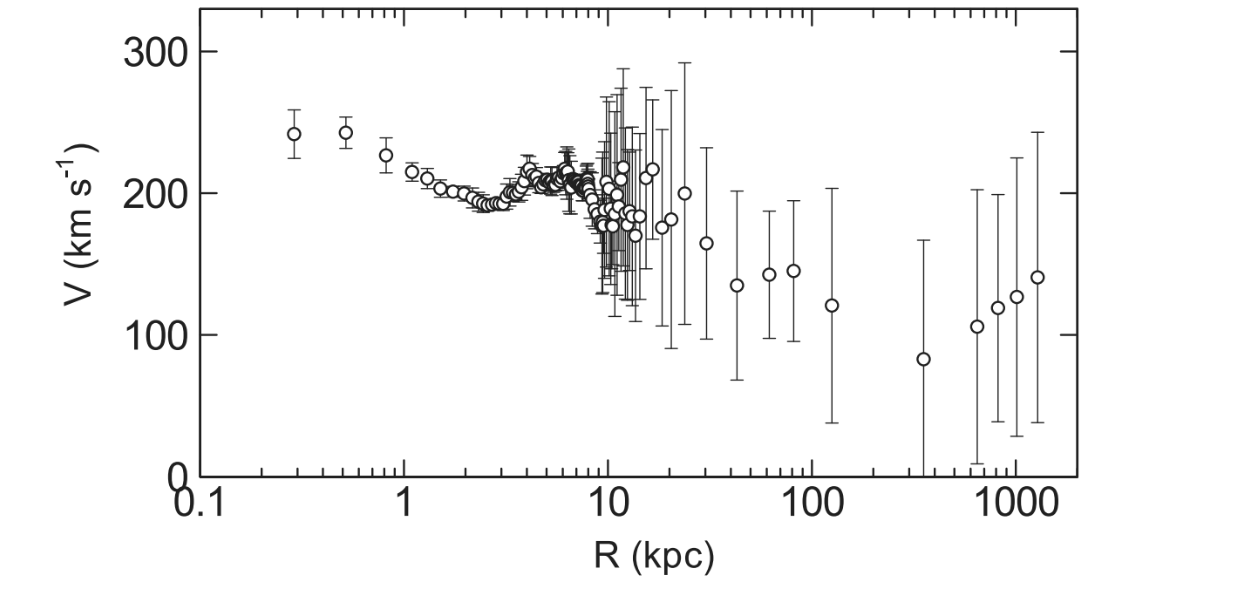
\includegraphics[width=\linewidth]{Sofue_MWtoLGData}
    \caption{Milky Way rotation curve data from radio signals and SDSS CO star line shifts  \cite{Sof11}}
    \label{fig:mwSofue}
\end{figure}
%Sofue: We included the circular velocities from an SDSS blue stars analysis by Xue et al. (2008; their model 1) by correcting for a systematic difference in the veloc-ities of about 20 km s1, due to our V0 = 200 km s1 instead of their 220 km s1.
%ugggh. have to look at the first two papers to see what assumptions they make. 
%We decomposed the newest rotation curve into a de Vaucouleurs bulge, an exponential disk, and an isothermal dark halo (Sofue et al. 2009).
%OBS METHOD: 
%An inner rotation curve was obtained by a terminal-velocity method applied to radio line observations
% An outer rotation curve was obtained by combining the CO star line velocities and the optical distances
%and by the HI disk-thickness method
%de Vaucouleurs bulge of mass Mb = 1.8 1010 Mˇ with a scale radius of Rb = 0.5 kpc, an exponential disk of mass Md = 71010Mˇ with a scale radius of Rd = 3.5 kpc,
%In the inner Galaxy at R .10 kpc, the rotation velocity is predominantly determined by the bulge and disk contributions, and R < 0.5 kpc it is almost determined by the bulge alone.


  We test the RCFM against three MW models;  a hybrid model from \citet{Xue} and \citet{Sofue}, a model from Stacy McGaugh, and one from (?) Mario Juric, as summarized in Table ~\ref{tab:my_label}.
  
   \begin{table*}[h!]
      \centering
      \begin{tabular}{|c|c|c|}
      \hline
        Author & Position of the Solar system   &  scalelength disk\\
        \hline
        Sofue \cite{sofue2009unified,10.1093/pasj/61.2.153,Sof11}   & 8 kpc &\\
             \hline
        McGaugh\cite{2021DDA....5240103M} & &\\
         \hline
        Klypin&&\\
         \hline
        Enbang Li&&\\
         \hline
      \end{tabular}
      \caption{Citations}
      \label{tab:my_label}
  \end{table*}
  
 

 


 








 
\subsection{  Geometry  and  Mass-to-light ratios}

 
  
    It is commonly assumed that   the stellar bulge, gas halo and   dark matter halo are spherically symmetric, but that the stellar disk is axially symmetric \cite{1954AJ.....59..273S}. 
    However, the assumption of spherical symmetry is commonly used   in evaluation of the   rotation curve velocities from integrated potentials \cite{2022A&A...664A..40M,PhysRevD.70.083509}, because numerical integration of the disk is a computationally intensive choice, and requires assumptions of  boundary conditions,   relevant physical scales,  etc. which add extra free-parameters\cite{2011A&A...531A..36H}.
Use of the spherically symmetric construction in the inner region of a galaxy $r< R_e/3$,  overestimates the potential of the thin disk by $30-45\%$ but maintains the same descending line shape and they converge for lengths $r>R_e/3$ where dark matter becomes important (see Fig.~\ref{fig:my_geom}).   This is   because flattened disks produce gravitational potentials which are weaker than a sphere of the same mass inside of $r< R_e/3$ \cite{Chatterjee}.


The spherical assumption we use is that of the 
 Schwarzschild metric, and spherical integration of the disk potential.   This overestimate  is reflected in our M/L ratios,   which can be scaled down to regain the disk potential.   This is the region where dark matter is not required to reproduce the rotation curve \cite{1985ApJAlbada}.   It is interesting to note that     the majority of introduced  error come from uncertainties in the M/L ratios, rather than the geometry assumptions \cite{2016Lelli}. 
 
 
\begin{figure}
    \centering
     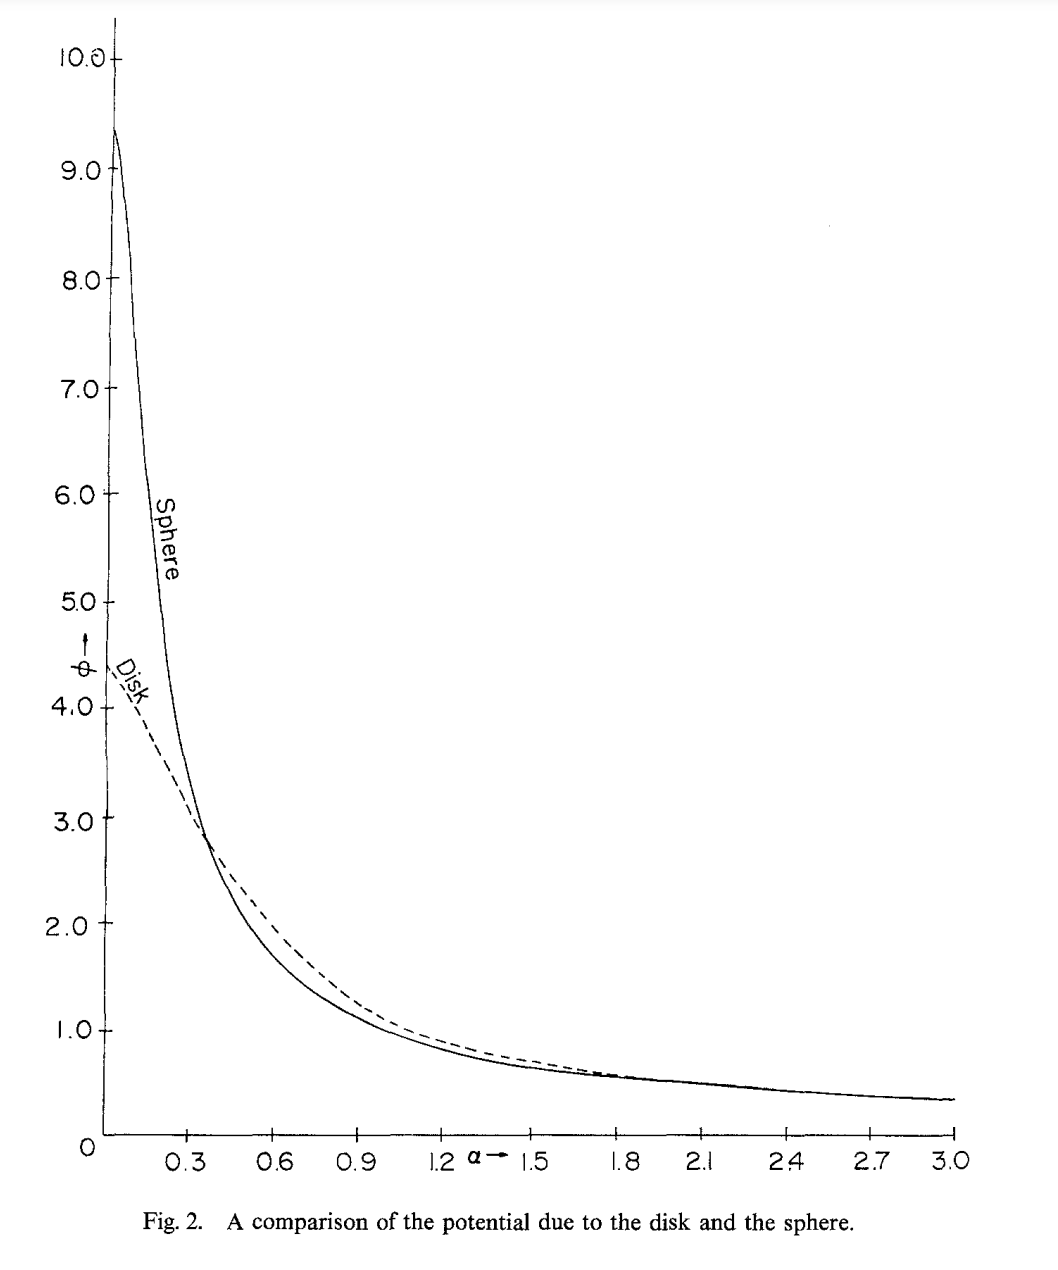
\includegraphics[width=\linewidth]{Chatterjee_SphereDisk.png}
    \caption{ $\alpha = r/R$, for $R$ the radial extent of the stars \cite{Chatterjee}}
    \label{fig:my_geom}
\end{figure}

 
 
    
 
   

% Please add the following required packages to your document preamble:
% \usepackage[table,xcdraw]{xcolor}
% If you use beamer only pass "xcolor=table" option, i.e. \documentclass[xcolor=table]{beamer}
\begin{table*}[]
\begin{tabular}{|l|r|r|r|r|}
\rowcolor[HTML]{FFE599} 
 \hline \hline
Galaxy                 & \multicolumn{1}{l}{\cellcolor[HTML]{FFE599}chi\_square} & \multicolumn{1}{l}{\cellcolor[HTML]{FFE599}alpha} & \multicolumn{1}{l}{\cellcolor[HTML]{FFE599}gamma\_disk} & \multicolumn{1}{l}{\cellcolor[HTML]{FFE599}gamma\_bulge} \\
 \hline \hline
UGCA442\_rotmod        & 0.546664313                                             & 152.0798352                                       & 2.285186637                                             & 1                                                        \\
UGC04305\_rotmod       & 1.552163817                                             & 1.13E-08                                          & 0.875530186                                             & 1                                                        \\
NGC2841\_rotmod        & 1.29859523                                              & 1.19564552                                        & 0.8692007195                                            & 1.105158794                                              \\
UGC07232\_rotmod       & 0.1892985827                                            & 938.617846                                        & 0.8198863754                                            & 1                                                        \\
NGC4068\_rotmod        & 0.1376258626                                            & 817.7792356                                       & 0.7987202945                                            & 1                                                        \\
D564-8\_rotmod         & 0.0563177862                                            & 2416.463117                                       & 1.216180048                                             & 1                                                        \\
NGC0024\_rotmod        & 0.6486941553                                            & 5.891641796                                       & 1.388640744                                             & 1                                                        \\
DDO168\_rotmod         & 3.086989612                                             & 737.2179381                                       & 0.788102085                                             & 1                                                        \\
UGC00128\_rotmod       & 5.325528279                                             & 8.411840984                                       & 1.646342074                                             & 1                                                        \\
D631-7\_rotmod         & 0.2418987957                                            & 1570.573781                                       & 0.2838910742                                            & 1                                                        \\
UGC01281\_rotmod-Copy1 & 0.2991971228                                            & 342.3372282                                       & 1.425626161                                             & 1                                                        \\
NGC2976\_rotmod        & 0.4109470835                                            & 24.00152827                                       & 0.9082215334                                            & 1                                                        \\
NGC6946\_rotmod        & 1.681620536                                             & 1.613701077                                       & 0.6410150758                                            & 0.5735330606                                             \\
NGC7331\_rotmod        & 0.9616636164                                            & 1.691051469                                       & 0.5128367912                                            & 1.201353002                                              \\
NGC5907\_rotmod        & 6.767970418                                             & 1.466981293                                       & 0.9342180305                                            & 1                                                        \\
NGC3198\_rotmod        & 1.676026322                                             & 5.002545411                                       & 0.8778064572                                            & 1                                                        \\
NGC0891\_rotmod        & 2.982570212                                             & 1.888876157                                       & 0.4153018842                                            & 0.7485043087                                             \\
NGC3741\_rotmod        & 0.5461975832                                            & 3793.870993                                       & 0.7236906274                                            & 1                                                        \\
NGC0247\_rotmod        & 1.925157677                                             & 4.731628756                                       & 1.525758435                                             & 1                                                        \\
UGC07524\_rotmod       & 1.343970708                                             & 19.78602906                                       & 1.588536233                                             & 1                                                        \\
UGC07151\_rotmod       & 0.9541856317                                            & 18.89200202                                       & 1.15329121                                              & 1                                                        \\
UGC04483\_rotmod       & 0.3255297918                                            & 606.8576739                                       & 1.27753238                                              & 1                                                        \\
NGC0055\_rotmod        & 2.50774124                                              & 61.6585064                                        & 1.016112277                                             & 1                                                        \\
NGC2403\_rotmod        & 10.2026916                                              & 11.32592717                                       & 0.8646379911                                            & 1                                                        \\
ESO444-G084\_rotmod    & 0.2144181763                                            & 271.3744936                                       & 1.867761903                                             & 1                                                        \\
NGC6789\_rotmod        & 0.142623013                                             & 521.8910289                                       & 1.412926654                                             & 1                                                        \\
UGC08490\_rotmod       & 0.1454390944                                            & 23.51044091                                       & 1.269505857                                             & 1                                                        \\
UGC07559\_rotmod       & 0.1211486206                                            & 626.6218015                                       & 0.9726082773                                            & 1                                                        \\
NGC2915\_rotmod        & 0.5819274509                                            & 464.9678164                                       & 0.5694400663                                            & 1                                                        \\
NGC5055\_rotmod        & 6.028325458                                             & 1.379543007                                       & 0.6199891339                                            & 1                                                        \\
NGC6503\_rotmod        & 1.418278403                                             & 9.753433142                                       & 0.7508894289                                            & 1                                                        \\
PGC51017\_rotmod       & 1.156258602                                             & 5.56E-08                                          & 0.8004543773                                            & 1                                                        \\
NGC1705\_rotmod        & 0.09524619526                                           & 21.00539942                                       & 1.254235701                                             & 1                                                        \\
UGC07577\_rotmod       & 0.03715559187                                           & 2778.757566                                       & 0.6696682482                                            & 1                                                        \\
NGC0300\_rotmod        & 0.3735595366                                            & 49.44834067                                       & 1.144934148                                             & 1                                                        \\
NGC7793\_rotmod        & 0.7005376378                                            & 7.612328582                                       & 0.8895669073                                            & 1                                                        \\
NGC4214\_rotmod        & 0.925101289                                             & 25.33456308                                       & 1.015914456                                             & 1                                                        \\
UGC08837\_rotmod       & 0.4323881041                                            & 832.4473126                                       & 0.7864452872                                            & 1                                                        \\
UGC07866\_rotmod       & 0.04035913416                                           & 195.9614021                                       & 1.261232793                                             & 1                                                        \\
UGC08286\_rotmod       & 2.180073076                                             & 21.43612788                                       & 1.662509956                                             & 1                                                        \\
NGC2683\_rotmod        & 0.7368400942                                            & 1.130098838                                       & 0.8843100202                                            & 0.4235079131                                             \\
IC2574\_rotmod         & 2.098089222                                             & 514.3585835                                       & 1.105464192                                             & 1                                                        \\
UGCA444\_rotmod        & 0.08902872741                                           & 251.8922167                                       & 3.78526637                                              & 1                                                        \\
NGC3109\_rotmod        & 0.2448564625                                            & 386.595152                                        & 2.054239954                                             & 1                                                        \\
DDO154\_rotmod         & 8.155263354                                             & 901.9180264                                       & 1.196264436                                             & 1                                                        \\
UGCA281\_rotmod        & 0.1579928991                                            & 203.5519405                                       & 1.23210673                                              & 1                                                        \\
CamB\_rotmod           & 0.1451570114                                            & 14949.63203                                       & 1.43E-05                                                & 1                                                        \\
NGC7814\_rotmod        & 0.5328768864                                            & 1.203771633                                       & 0.418848533                                             & 0.6735053081                                             \\
NGC2366\_rotmod        & 2.108042136                                             & 260.887004                                        & 1.06298292                                              & 1                                                        \\
\end{tabular}
 \hline \hline
  \caption{RCFM results, Training Set
      }
   \label{tab:Tset2}
\hline
\end{table*}
 
%%%%%%%%%%%%%%%%%%%%%%%%%%%%%%%%%%%%%%%%%%%%%%%%%%%%%%%%%%%%%%%%%%%%%%%%%%%%%%%%%%%%%%%%%%%%%%%%
%%%%%%%%%%%%%%%%%%%%%%%%%%%%%%%%%%%%%%%%%%%%%%%%%%%%%%%%%%%%%%%%%%%%%%%%%%%%%%%%%%%%%%%%%%%%%%%%%%%%
%%%%%%%%%%%%%%%%%%%%%%%%%%%%%%%%%%%%%%%%%%%%%%%%%%%%%%%%%%%%%%%%%%%%%%%%%%%%%%%%%%%%%%%%%%%%%%%%%%%%%%
%%%%%%
%%%%%%%%%%%%%%%%%%%%%%%%%%%%%%%%%%%%%%%%%%%%%%%%%%%%%%%%%%%%%%%%%%%%%%%%%%%%%%%%%%%%%%%%%%%%%%%%%%%%%%%
\section{Analysis and Constraining the free parameter \label{sec:analysis}}
 
 
In RCFM fits reported here, the    bulge and disk mass-to-light ratios are allowed to vary freely from $1.0$ (See Eq.~\ref{eq:zonte3}), and the average resulting fit values are within stated criteria    of $\pm 20\%$ \cite{2016Lelli}. The gas fractions (HI scaled for Helium abundance) are fixed,  though addition of molecular gas could increase mass fractions in the inner kiloparsec of a galaxy   \cite{2004ApJ...609..652M}.


\subsection{NGC 3198 and other galaxies(UNDER CONSTRUCTION)}
\cite{1985ApJAlbada} studies this galaxy, which MOND has troubles with. This galaxy has   a thin exponential disk (de Vaucouleurs 1959),
(Freeman 1970).  
 
\cite{Toky} mentions that MOND fails to fit NGC 3109, which we fit exceedingly well ($\chi^2 = 0.32$).

NGC 2841 is also a problem for MOND
%%%%%%
%%%%%%%%
%%%%%%
%%%%%%%
%%%%%%
%%%%%%
\subsection{Correlation to  the model's free parameter }

To constrain a guess at a functional interpretation of the model's free-parameter, we select a
  subset of galaxies in Table~\ref{tab:Tset2}. The  subset is selected based on
   galaxies that have highly accurate distance:   tip of the red giant branch,  Cepheids, and  from supernova, with errors in distance on the order of $5\% - 10\%$ \cite{2016Lelli}. Of these, We   exclude galaxies  which have an inclination greater than $85^o$ as impossible to constrain a proper surface brightness profile, and those at inclinations less than $35^o$ as being impossible to accurately report line of sight Doppler shifts.  We also reject  three galaxies with significant non-circular motions and poor quality factors in the SPARC database.  
  By this process, we select 43 galaxies (See Table \ref{tab:Tset}). 
  
  
  \begin{table*}[]
      \centering
      \begin{tabular}{|c|c|c|c|c|c|}
      \hline \hline
Galaxy Name & Hubble Type(1)& 	Distance (Mpc)&Mean Error on D (Mpc)& 	Distance Method (2)& 	Inc (deg)\\
    \hline \hline\\
CamB&   	10&    3.36&  	0.26&   2&  65\\
D564-8& 	10& 	8.79& 	0.28& 	2& 	63\\
D631-7& 	10& 	7.72& 	0.18& 	2& 	59\\
DDO154& 	10& 	4.04& 	0.2& 	2& 	64\\
DDO168& 	10& 	4.25& 	0.21& 	2& 	63\\
ESO444-G084& 10& 	4.83& 	0.48& 	2& 	32\\
IC2574& 	9& 	3.91& 	0.2&    	2& 	75\\
NGC0024& 	5& 	7.3& 	0.36&   	2& 	64\\
NGC0055& 	9& 	2.11& 	0.11&   	2& 	77\\
NGC0247& 	7& 	3.7& 	0.19&   	2& 	74\\
NGC0300& 	7& 	2.08& 	0.1&    	2& 	42\\
NGC0891& 	3& 	9.91& 	0.5&    	2& 	90\\
NGC1705& 	11& 	5.73& 	0.29& 	2& 	80\\
NGC2366& 	10& 	3.27& 	0.16& 	2& 	68\\
NGC2403& 	6& 	3.16& 	0.16&   	2& 	63\\
NGC2683& 	3& 	9.81& 	0.49&   	2& 	80\\
NGC2841& 	3& 	14.1& 	1.4&    	3& 	76\\
NGC2915& 	11& 	4.06& 	0.2& 	2& 	56\\
NGC2976**& 	5& 	3.58& 	0.18&   	2& 	61\\
NGC3109& 	9& 	1.33& 	0.07&   	2& 	70\\
NGC3198& 	5& 	13.8& 	1.4&    	3& 	73\\
NGC3741& 	10& 	3.21& 	0.17& 	2& 	70\\
NGC4068& 	10& 	4.37& 	0.22& 	2& 	44\\
NGC4214& 	10& 	2.87& 	0.14& 	2& 	15\\
NGC5055& 	4& 	9.9& 	0.3&    	2& 	55\\
NGC5907& 	5& 	17.3& 	0.9&    	2& 	88\\
NGC6503& 	6& 	6.26& 	0.31&   	2& 	74\\
NGC6789& 	11& 	3.52& 	0.18& 	2& 	43\\
NGC6946& 	6& 	5.52& 	1.66&   	2& 	38\\
NGC7331& 	3& 	14.7& 	1.5&    	3& 	75\\
NGC7793& 	7& 	3.61& 	0.18&   	2& 	47\\
NGC7814& 	2&  	14.4& 	0.66& 	2& 	90\\
PGC51017**& 	11& 	13.6& 	1.4& 	2& 	66\\
UGC01281& 	8&   	5.27& 	0.24& 	2& 	90\\
UGC04305**& 	10& 	3.45& 	0.17& 	2& 	40\\
UGC04483& 	10& 	3.34& 	0.31& 	2& 	58\\
UGC07151& 	6& 	6.87& 	0.34&   	2& 	90\\
UGC07232& 	10& 	2.83& 	0.17& 	2& 	59\\
UGC07524& 	9& 	4.74& 	0.24& 	    2& 	46\\
UGC07559& 	10& 	4.97& 	0.25& 	2& 	61\\
UGC07577& 	10& 	2.59& 	0.13& 	2& 	63\\
UGC07866& 	10& 	4.57& 	0.23& 	2& 	44\\
UGC08286& 	6& 	6.5& 	0.21&   	2& 	90\\
UGC08490& 	9& 	4.65& 	0.53&   	2& 	50\\
UGC08837& 	10& 	7.21& 	0.36& 	2& 	80\\
UGCA281& 	11& 	5.68& 	0.28& 	2& 	67\\
UGCA442& 	9& 	4.35& 	0.22& 	    2& 	64\\
UGCA444& 	10& 	0.98& 	0.05& 	2& 	78\\
    \hline \hline           
      \end{tabular}
      \caption{Table from  \citet{2016Lelli}. 
      (1) Hubble type:  from (CITE) de
Vaucouleurs et al. (1991), (CITE) Schombert et al. (1992), or (CITE) NED3
of: 0 = S0, 1 = Sa, 2 = Sab,
3 = Sb, 4 = Sbc, 5 = Sc, 6 = Scd, 7 = Sd, 8 = Sdm,
9 = Sm, 10 = Im, 11 = BCD.  (2) Distance method: : 1 = Hubble flow,
2 = tip of the red giant branch, 3 = Cepheids, 4 = Ursa Major
cluster of galaxies, 5 = supernovae. ** notes galaxies excluded from fit bc fail to fit, and see if we want to include SN gals, there's only 3...and 2 of the 3 that fail are weirdi rotations (non-circular)}
0      \label{tab:Tset}
  \end{table*}
  
  %%NOTE: Homies for SPARC used hybrid rotation curves on 56 galaxies, combining H-alpha  (inner) with HI (outer) Check if our "bad" gals are part of thi, or if is algo mas. Despite the high spatial resolution, Hα rotation curves are sometimes quite uncertain due to the patchy distribution and complex kinematics of Hα gas, especially for low-mass and LSB galaxies. We %use only H I data for the several objects:DDO 154, IC 2574, NGC 3109, NGC 5033, NGC 5055,NGC 6946, NGC 7331, and UGC 2259.(THESE ARE ALL GOOD
 
%or face-on ones.We assign a quality flag (Q) to each rotation curve using the following scheme: Q = 1 for galaxies with high-quality H I data or hybrid Hα/H I rotation curves (99 objects); Q = 2 for
%galaxies with minor asymmetries and/or H I data of lower
%quality (64 objects); Q = 3 for galaxies with major asymmetries, strong noncircular motions, and/or offsets between H I
%nd stellar distributions (12 objects). Galaxies with Q = 3 are%
%not suited for detailed dynamical studies: we build mass models
%for completeness but do not consider them in our analysis.
%K BIEN_ Both UGC04305_rotmod and PGC51017_rotmod have Q=3. discard anyhow. but not: NGC2976_rotmod, it's a Q=2. Plus we have a few other galaxies in this subset with a Q=3,,,


  We the  $\alpha$ values of the subset versus a proxy for the gradient in the gravitational potential
  
   \begin{equation}
     \rho = L_{total}/R_{eff}.
 \end{equation}
 
 The  estimates of the  total luminosities $L_{total}$ at $3.6 \mu m$,  assume a solar
absolute magnitude of 3.24 at $3.6 \mu m$ (CITE Oh et al. 2008). The effective radius $R_{eff}$ is    the radius encompassing half of the total luminosity \citet{2016Lelli}.  We find $\alpha$  to be   strongly correlated to  this quantity, with 
\begin{equation}
    \alpha = 54.3 (L/R_e)^{-1.09}
\end{equation}

at a confidence f $83.3\%$, see Fig.~\ref{alpha2}.
  
 \begin{figure}[h]
%\scalebox{0.5}%
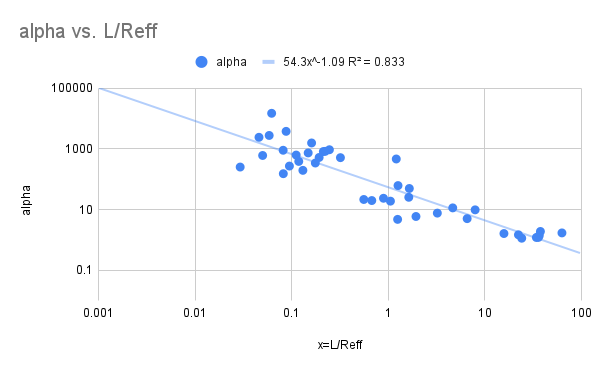
\includegraphics[width=\linewidth]{alphavL_Reff.png} 
\caption{  Free-parameter correlation   }
\label{alpha2}
\end{figure}  
 


We might assume that $\alpha$ is a ratio of the same quantity for  the Milky Way $\rho_{mw}$ with respect to the other   galaxy $\rho_{gal}$  

\begin{equation}
\alpha=\left(\frac{\rho_{mw}}{\rho_{gal}}\right)^{b}  ,
\label{correl}
\end{equation}

as other quantities in this formalism.
 
\subsection{MOND  \& RAR Comparison}

While reported error    estimates on rotation curve velocities  have not been standardized across the field~\citep{Blok,Gent},     one can reliably   compare fits to the same data with the same  errors. The     reduced $\chi^2_r$ values in table (REF TABLE), demonstrates that the RCFM reduced $\xi^2$ values are twice as low on average as those of the RAR fits  \cite{McGaugh2016RAR}  .

 
 
 \section{  Conclusions \label{sec:conclu}  }
 

{\color{red} This heuristic replacement of dark matter is not a fundamental derivation, but    one supposes if it is possible to quantify these
excesses in shifted spectra using only luminous mass as we do in this paper,  then a       derivation from first principles should   exist.  The curious conspiracy of the luminous mass to   determine the dark matter  is here more compactly explained and characterized as the imprint of our Milky Way on Doppler shifted spectra we receive from external galaxies. Not only is this a more efficient way to predict rotations curves as judged by the average reduced $\chi^2$, but it is also a  more conservative choice than either MOND or dark matter which both require new physics \cite{de_Blok_2010}.  
  
 
 

  
 
%Places where dark matter is invoked. Structure formation: put spherical model replace flat, solve. Galaxy clusters, same,put flow lines on surfaces supported by dark energy. Tully Fisher: temp dependence with mass - but read Beckenstein's description carefully. Hemakes some points.  
   
 
We   present here a new picture of flat-rotation curves which does not   modify Einstein gravitational physics, but adds a new technique to the standard transformations of   relativity. It is falsifiable if dark matter is found to be necessary in our Milky Way.   Recent large surveys of millions of  stars in the Milky Way will differentiate these models     \cite{2022ApJS..259...35A}, \cite{2010ApJ...716....1B}.
  }
  
  % We propose   that the other places  where dark matter is invoked     require more complicated  physics assumptions 
      %than are presented here; and can be informed by observations of large scale flows 
     
      %,    and the ``too'' early   formation of galaxies 
     
     % Discrepancies in estimates of the Hubble Flow from supernovae versus from the cosmic microwave background (CITE) and (WHAT"S THE OTHER ISSUE YO). DO I want to include this? 
      
     % MOND      has a fascinating, compact explanation for another dark matter paradox, the  
  % Tully-Fisher relation \cite{1977A&A....54..661T,McGaugh_2000}, but that also is beyond the scope of the current work unfortunately.   
 %In example, the James Webb Space Telescope may have already falsified dark matter driven galaxy formation \cite{2022arXiv221014915H}.
   

%%%%%%
%%%%%
%%%
%%
%
%%%%%%


 % \caption{Results   for SPARC Luminous mass profiles  [NOT UPDATED]\label{sumRESULTS}}
 % \begin{tabular}{@{}llccccccc@{}}
 % \hline
 %  Galaxy     	  &Ref.~&  \multicolumn{3}{c}{\underline{ Other Model Fit Results}}	& & \multicolumn{3}{c}{\underline{LCM Fit Results }}  \\
%\hline
%   	 	& & &  $M/L_{disk}$		& $\chi^2_r$	&&$M/L$&$r_e$&$\chi^2_r$ \\ 
% \hline
%F 563-1	& 2	%& 			
%					&NFW	&--	 		&-- & 	&1.13 	&2.84 	&0.06 \\
%M 31* 	& 12 	%&7.5
%					&ISO	 	 &7.50		&0.36 & 	&5.88	 &4.80 	&0.04  \\
%M 33		& 5	 %&	K 		
%					& NFW 	&0.70		&2.46&  	 &1.98	 &1.46	& 0.17 \\
%NGC 891*	& 11 	% &3.6$\,\umu$m 
		%			&MaxLight &0.9 			&1.10  & 	 &--  	 &	&0.25 \\ 
%NGC 925 	&3	%&3.6$\,\umu$m
 			%		&ISO 	&0.18		 &2.40& 	&0.92	 &4.35	&0.11 \\
%NGC 2403	 & 3	%& 3.6$\,\umu$m
		%			& NFW	&0.41 	 	&4.56& 	&1.12	 	&2.18		& 0.88 \\
%NGC 2841*  &6-3	% & 3.6$\,\umu$m
%					&  James	&0.74 	 	&0.45 & 	&6.25	  &4.84	&0.11 \\
%NGC 2903  &10	 %&B	   		
%					&MOND   	&3.60 	 	&10.71& 	 &2.2	 	&2.81		&0.47\\
% NGC 3198 & 3 	%&3.6$\,\umu$m
%					 &NFW	&0.80	   	&5.40  &   	 &1.80 	 &5.10	&0.64   \\
%NGC 3521  & 8-6	 %&3.6$\,\umu$m 
%					&MOND	&0.71 	 	&0.97 & 	 &2.13  &3.23	&0.22 \\
%NGC 3726	& 10	%&B 			
%					&MOND	&1.00	 	&3.57& 	&1.06	 &2.70	&0.05 \\
%NGC 3953	& 10	%&B 			
%					&MOND	&2.7		 	&1.35& 	&1.79 	&2.60 	&0.35 \\
%NGC 3992	& 10	%&B 			
%					&MOND	&4.93	 	&0.50& 	&2.45 	 &4.77	&0.04 \\
%NGC 4088	& 10	%&B 			
%					&MOND	&1.16		 	&1.70& 	&5.58	 &2.70	&0.27 \\
%NGC 4138	& 10	%&B 			
%					&MOND	&3.5		 	&2.12& 	&3.67	 &1.46	&0.01 \\
%NGC 5055*	 & 3	%&3.6$\,\umu$m 
%					&  NFW	&0.79	 	&17.23&  	&5.87	 &3.29	&0.69 \\
%NGC 5533*	 & 10 %&B 			
%					&MOND	&0.6		  	&1.57 & 	&7.11 	  &3.23	&0.22  \\
%NGC 5907*	& 10	%&B 			
				%	&MOND	&1.6 		 	 &0.44& 	&2.04	 &3.45	%&0.09 \\
%NGC 6946*	&  10	 %& B			
%					&  MOND	& 0.5		 	&   3.03& 	&1.44 	 &0.76	&0.07  \\ 
%NGC 6946*	&  3	 %& B			
%					&  NFW	& 0.5		 	&   3.03& 	&1.44 	 &0.76	&0.07  \\ 
%NGC 7331	&8	% & 3.6$\,\umu$m
%					&James	&0.4 		 	& 0.45& 	&1.34	 &2.44	&0.09 \\
%NGC 7793  &14	%&B			
%					&ISO		&2.6		 	&1.08& 	&2.7	 &1.51	&0.11 \\
%NGC 7814* &11 	% & 3.6$\,\umu$m
%					&ISO   	& 0.68  	 	& 0.25& 	 &-- 	   &	&0.20 \\ 
%UGC 128		&6	%&				
	%				&James	&			&	&	&1.58	  &10.3	%&0.20\\
%UGC 6973	& 10	%&B 			
%					&MOND	&2.7		 	&23.5 & 	&--  	& 	&0.06 \\
%UGC 7524	& 6	%&B 			
%					&James	&--		 	&-- & 	&2.10 	&3.32 	&0.06 \\
% 1.~\citet{Bege}, 2.~\citet{JNav}, 3.~\citet{Blok} , 4.~\citet{Maria}, 
%5.~\citet{Cor03}, 6.~\citet{James},   7.~\citet{Batt},   8.~\citet{Gent},   9.~\citet{Bot},   10.~\citet{SanMcGa},
 % 11.~\citet{Frat},   12.~\citet{Car},   13.~\citet{giraud2000universal},   14.~\citet{Dicaire}, %15.~\cite{Klypin}. \\
%    \end{minipage}
%\end{table*} 


   

  \section[]{Acknowledgments}
 This work is dedicated to Emmett Till, with respect and gratitude to the first nations 
 on whose lands this was written; 
  the Coast Salish Peoples of Washington State, 
 the Cheyenne,
 Arapaho and Ute  Peoples of Colorado, and the Algonquian Peoples of Massachusetts.  

  The authors would like to thank  S.\ McGaugh,  V.\,P.\,  Nair,   R.\, Walterbos,  A.\, Klypin, K. Bender, C. Beetle and     T.\, Boyer.   \\
  
 
% QUESTION FOR GROUP: how is our model predictive, more so than MOND, since we both do well on fitting galaxies. The Milky Way. We get a large enough sample of galaxies with certain distances and good photometry (SPARC) and run against a two MW. 



 \begin{figure}[h]
\begin{subfigure}{.5\textwidth}
  \centering
  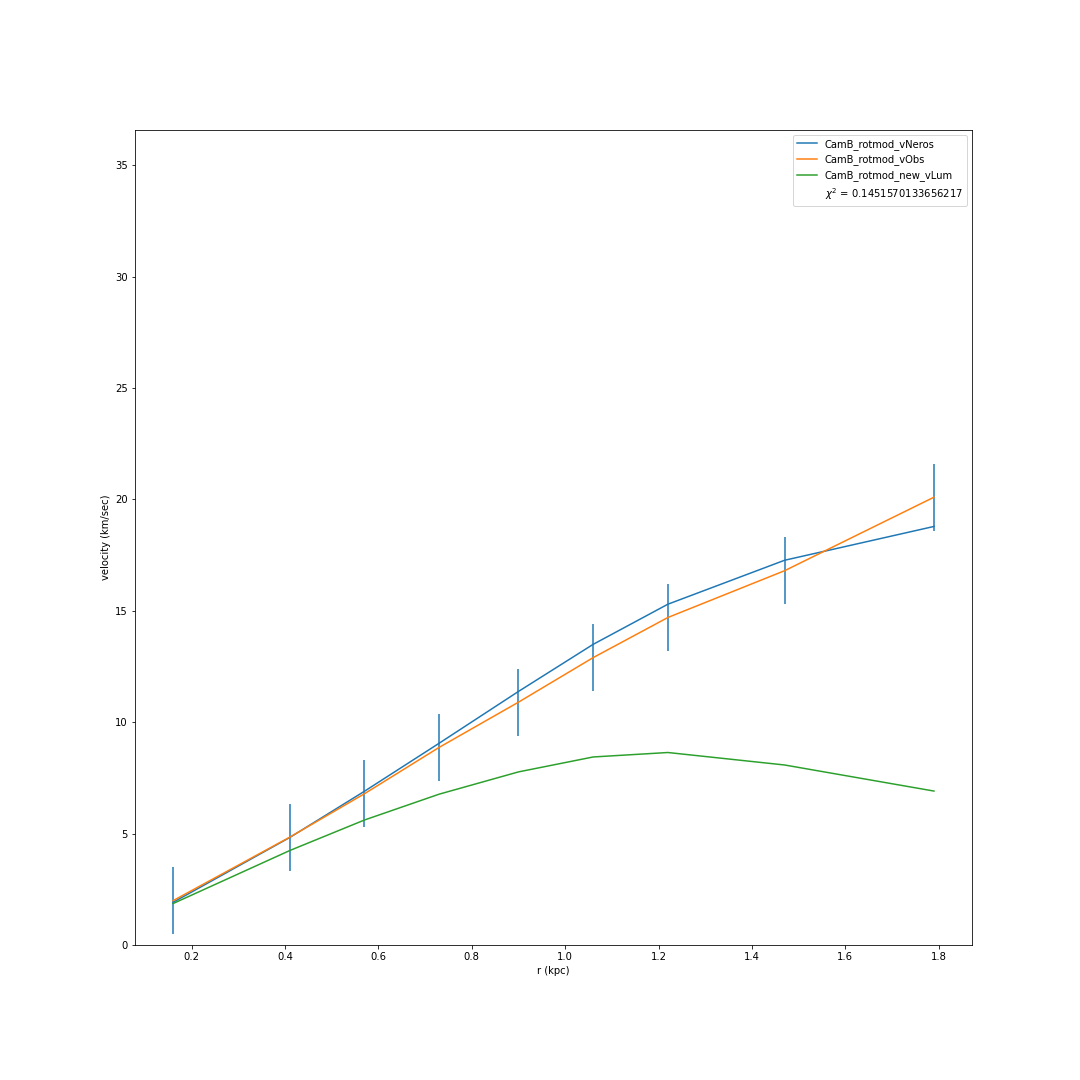
\includegraphics[width=.8\linewidth]{figures/CamB_rotmod_XueSofue.png}
  \caption{SPARC\cite{2016Lelli}}
  \label{fig:sfig1}
\end{subfigure}%
\begin{subfigure}{.5\textwidth}
  \centering
  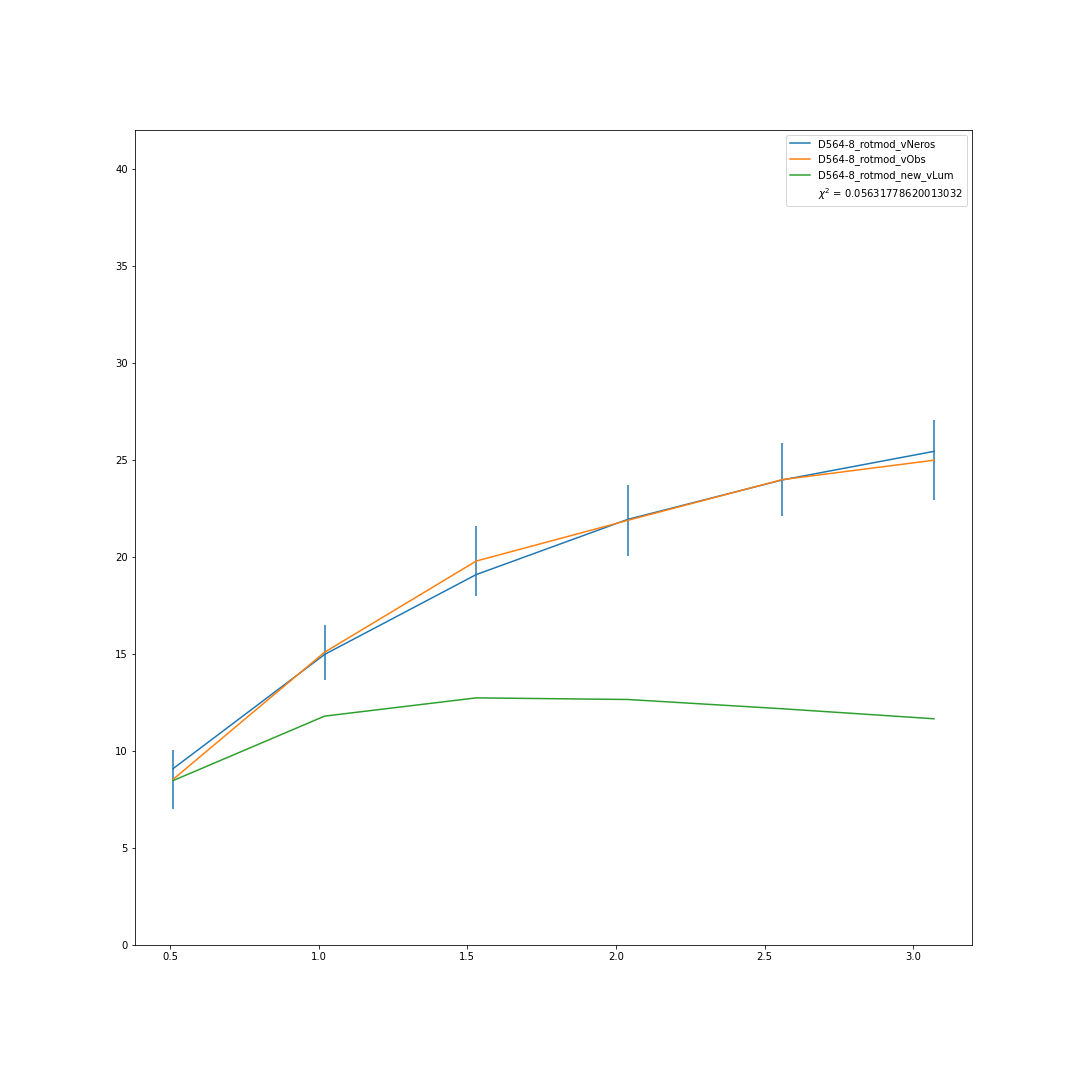
\includegraphics[width=.8\linewidth]{figures/D564-8_rotmod_XueSofue.png}
  \caption{D564-8}
  \label{fig:sfig2}
\end{subfigure}
\begin{subfigure}{.5\textwidth}
  \centering
  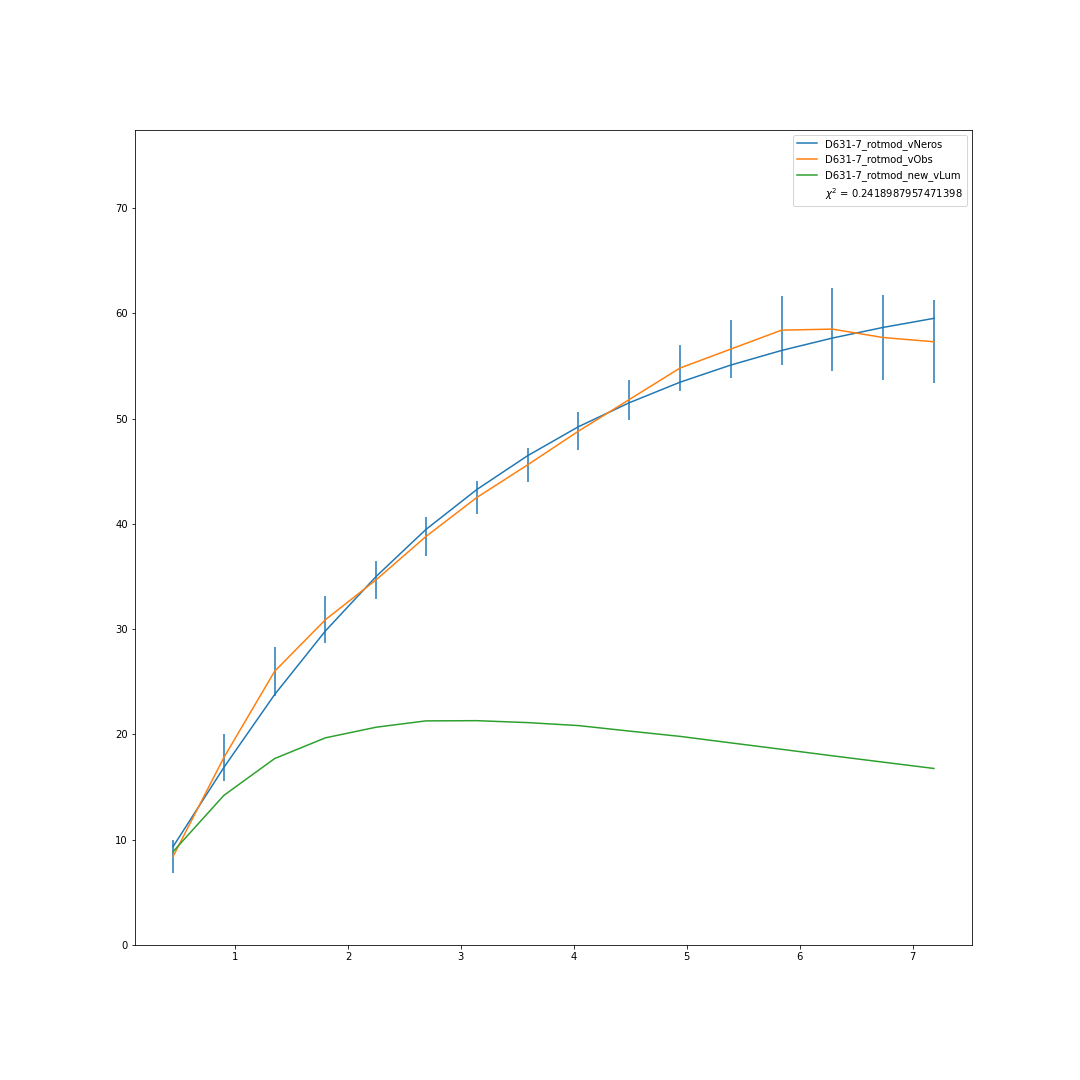
\includegraphics[width=.8\linewidth]{figures/D631-7_rotmod_XueSofue.png}
  \caption{D631-7}
  \label{fig:sfig3}
\end{subfigure}
\begin{subfigure}{.5\textwidth}
  \centering
  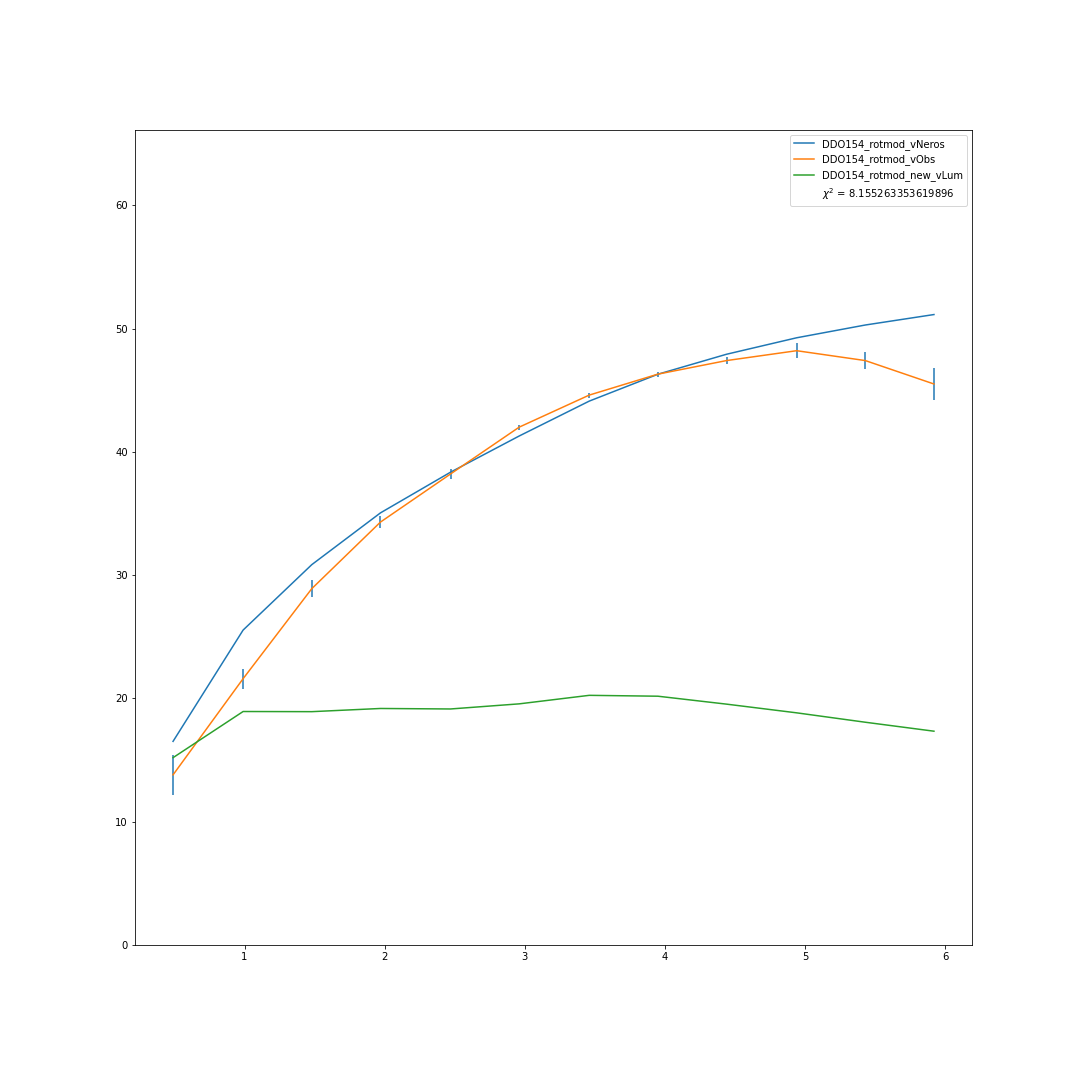
\includegraphics[width=.8\linewidth]{figures/DDO154_rotmod_XueSofue.png}
  \caption{DDO154}
  \label{fig:sfig4}
\end{subfigure}%
\begin{subfigure}{.5\textwidth}
  \centering
  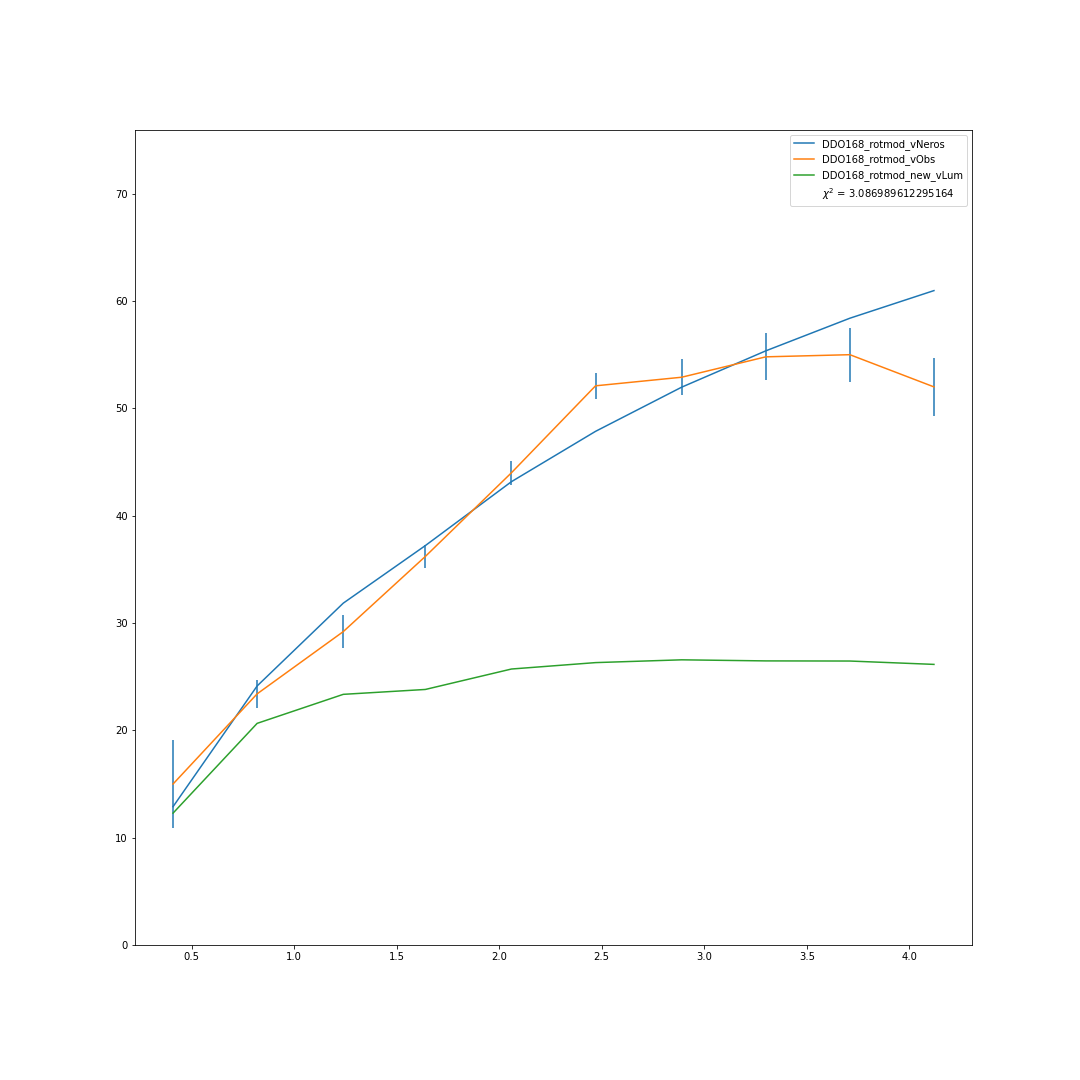
\includegraphics[width=.8\linewidth]{figures/DDO168_rotmod_XueSofue.png}
  \caption{DDO168}
  \label{fig:sfig5}
\end{subfigure}
\begin{subfigure}{.5\textwidth}
  \centering
  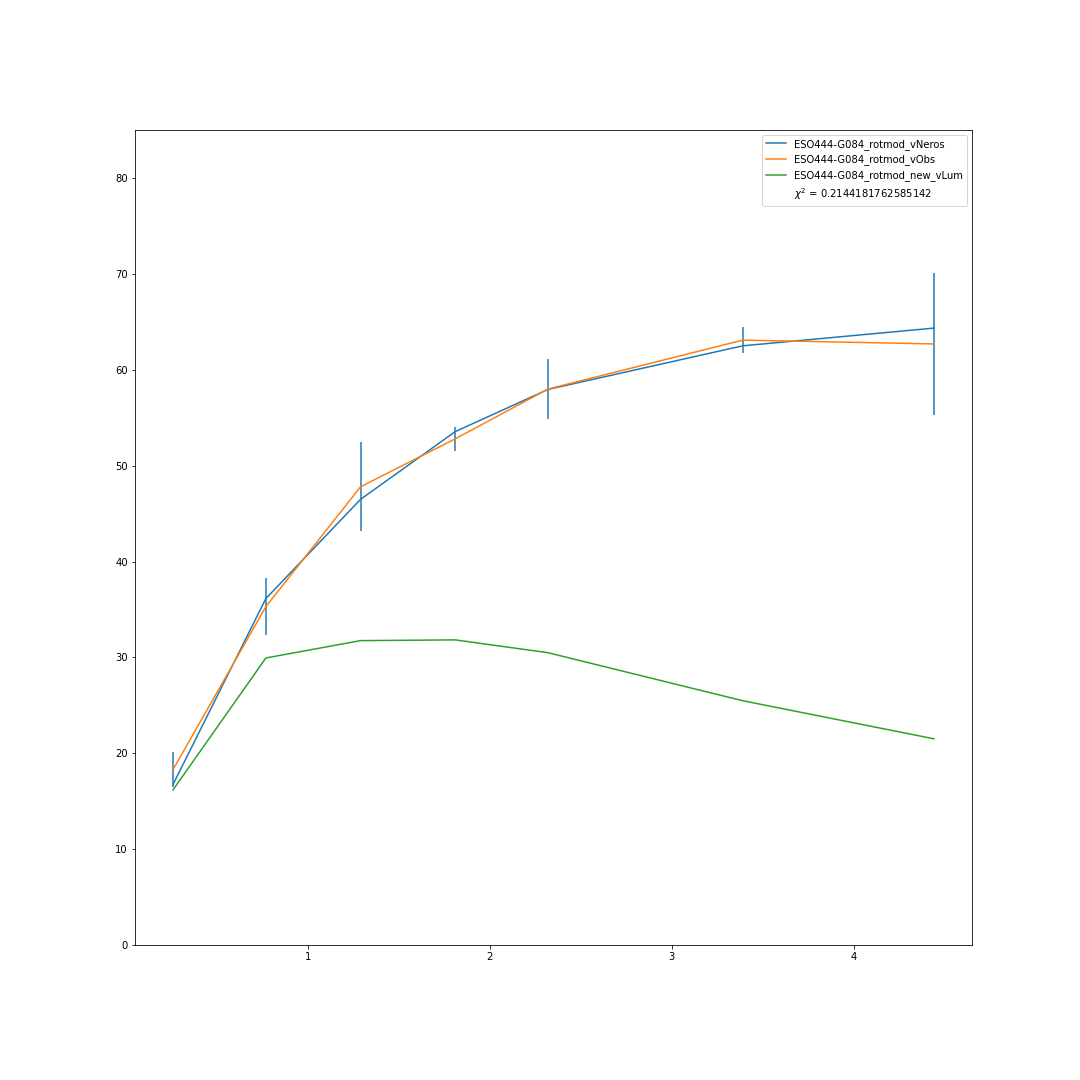
\includegraphics[width=.8\linewidth]{figures/ESO444-G084_rotmod_XueSofue.png}
  \caption{ESO444-G084}
  \label{fig:sfig9}
\end{subfigure}%
\end{figure}

\clearpage
  \begin{figure}[h]
\begin{subfigure}{.5\textwidth}
  \centering
  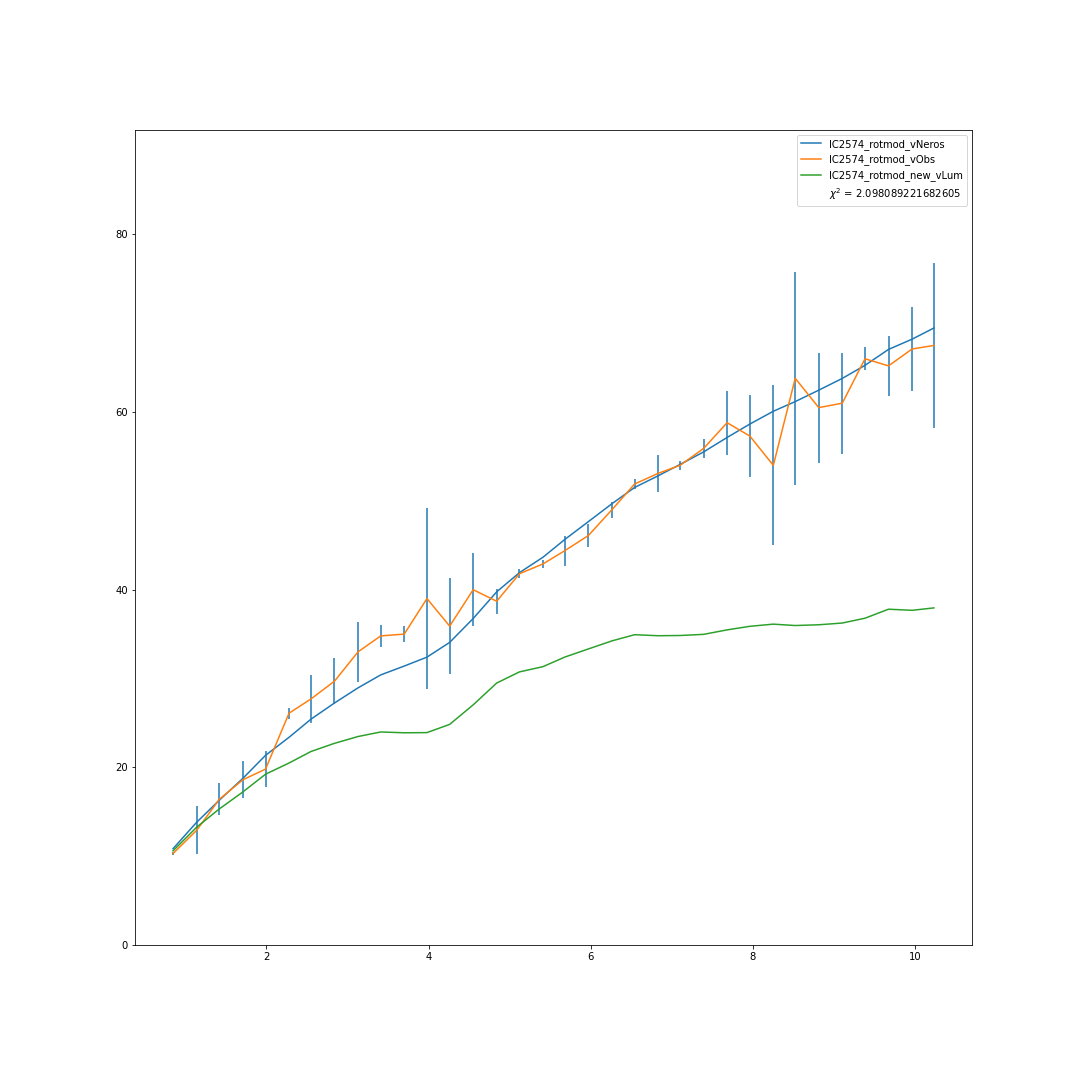
\includegraphics[width=.8\linewidth]{figures/IC2574_rotmod_XueSofue.png}
  \caption{IC2574}
  \label{fig:sfig10}
\end{subfigure}
\begin{subfigure}{.5\textwidth}
  \centering
  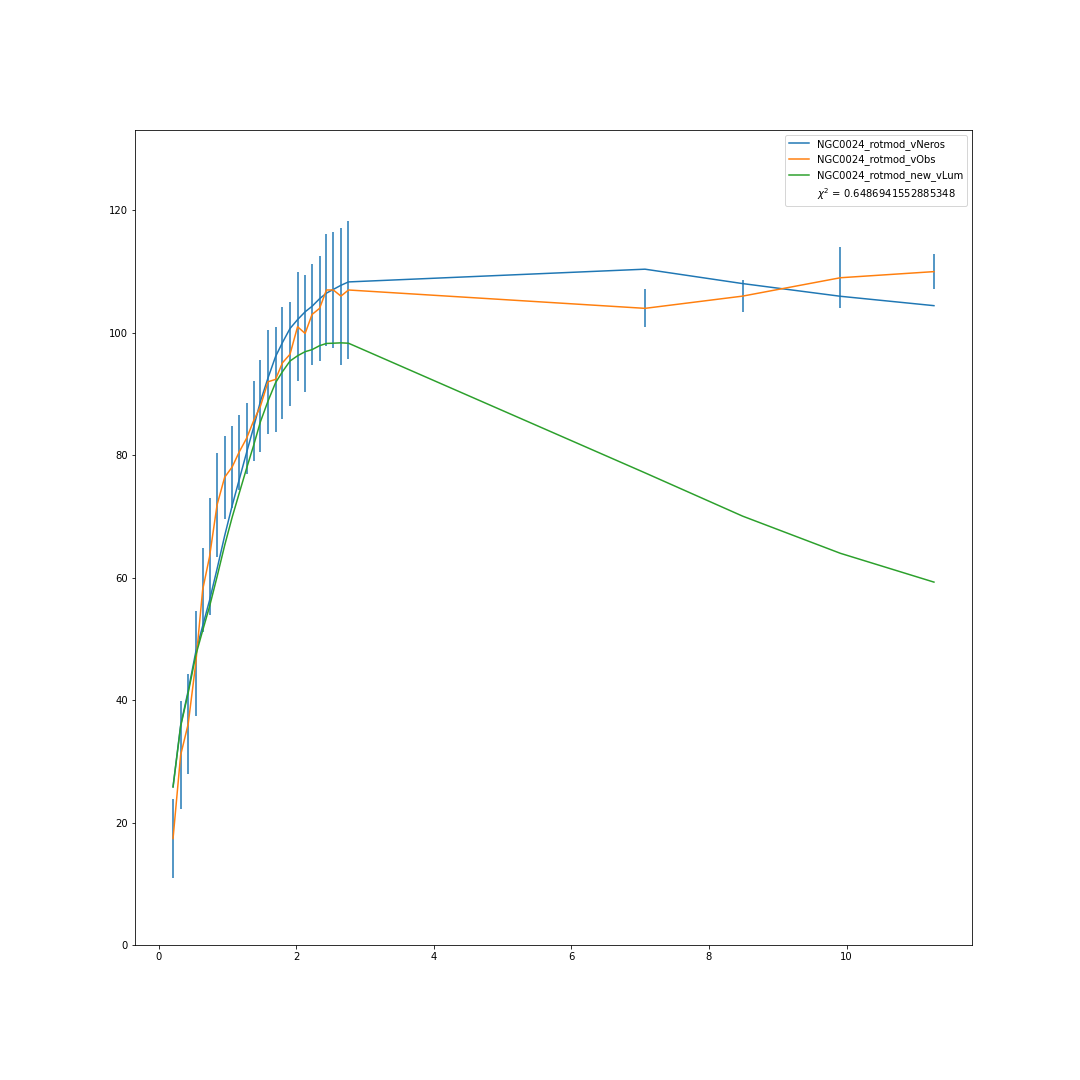
\includegraphics[width=.8\linewidth]{figures/NGC0024_rotmod_XueSofue.png}
  \caption{NGC0024}
  \label{fig:sfig6}
\end{subfigure}%
\begin{subfigure}{.5\textwidth}
  \centering
  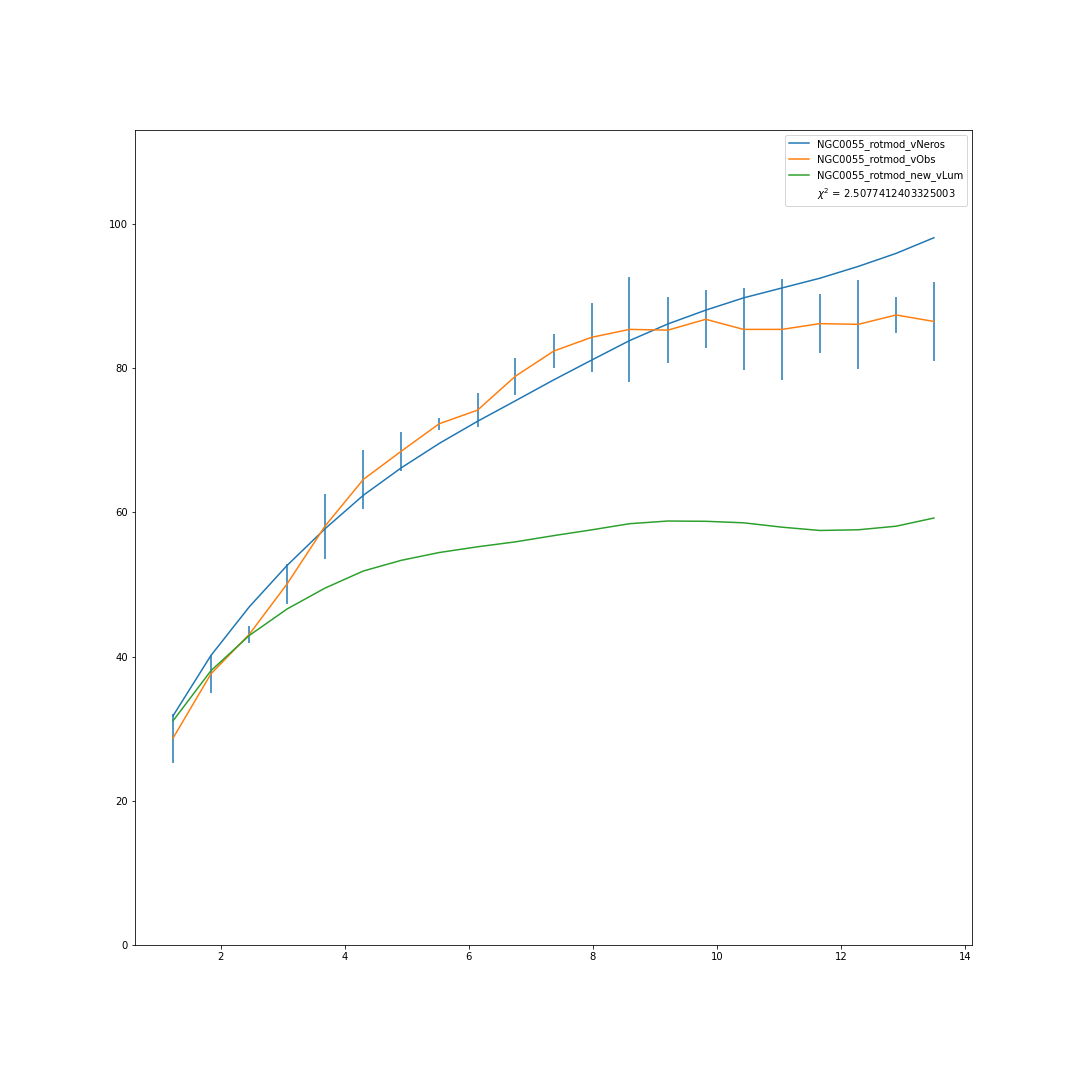
\includegraphics[width=.8\linewidth]{figures/NGC0055_rotmod_XueSofue.png}
  \caption{NGC0055}
  \label{fig:sfig7}
\end{subfigure}
\begin{subfigure}{.5\textwidth}
  \centering
  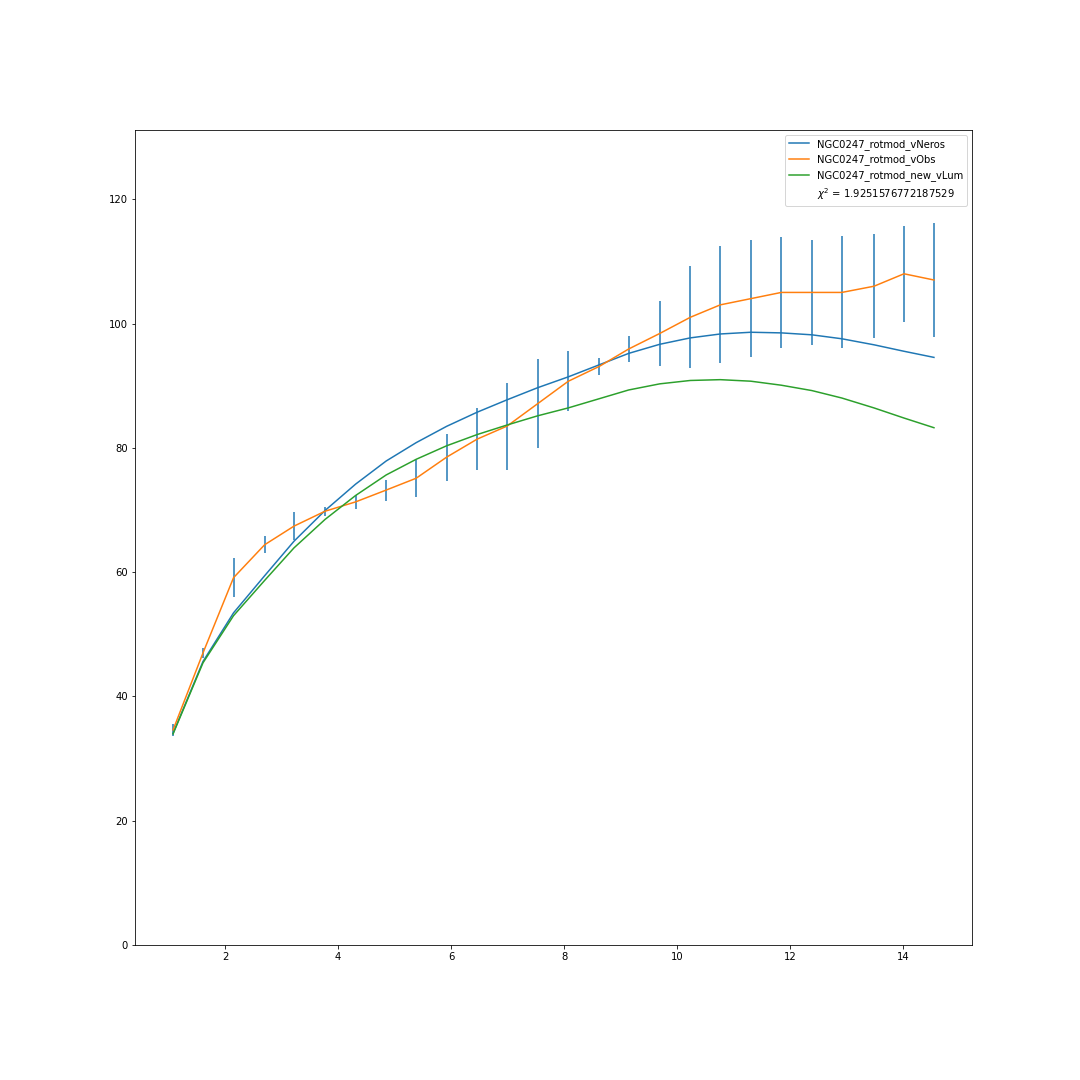
\includegraphics[width=.8\linewidth]{figures/NGC0247_rotmod_XueSofue.png}
  \caption{NGC0247}
  \label{fig:sfig8}
\end{subfigure}
\begin{subfigure}{.5\textwidth}
  \centering
  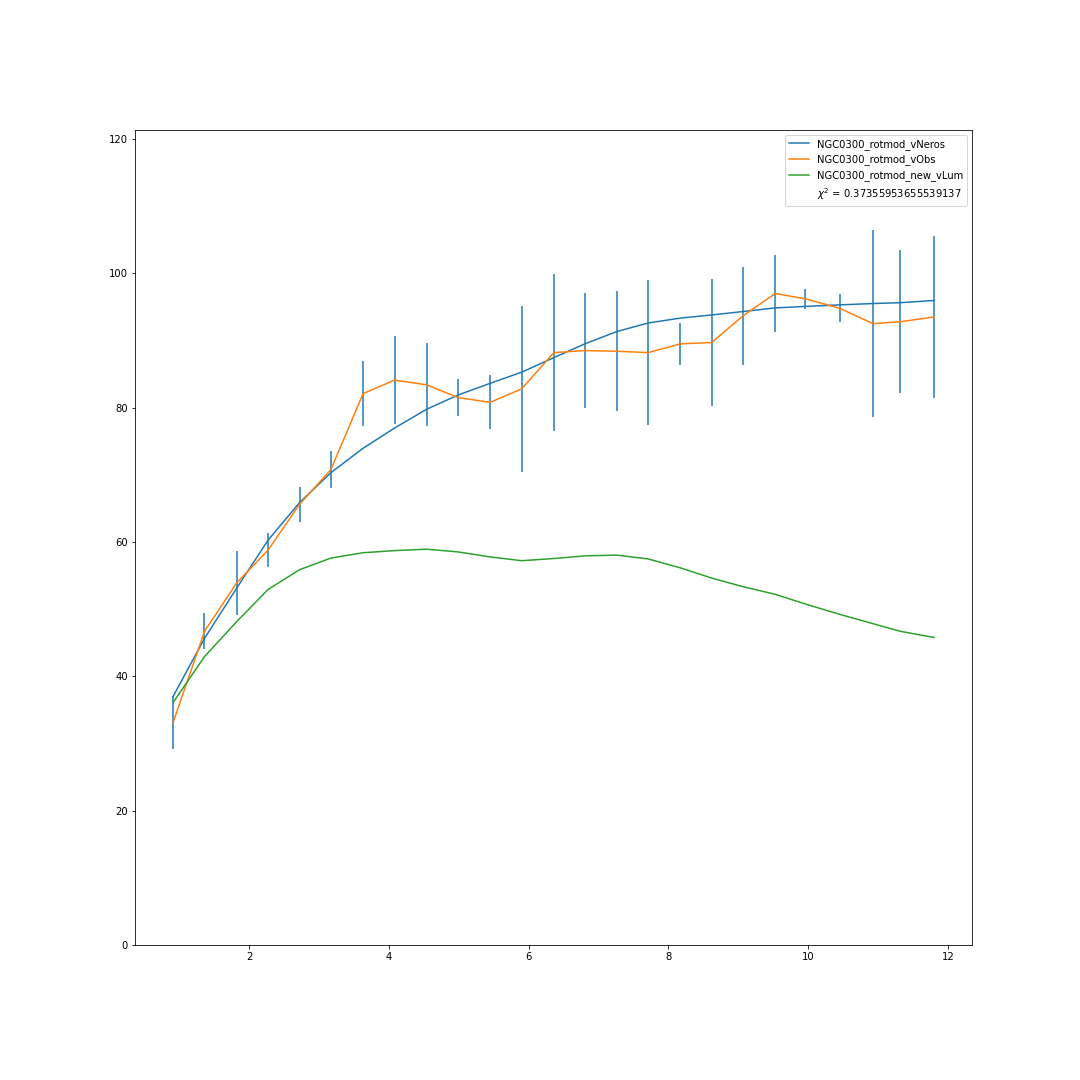
\includegraphics[width=.8\linewidth]{figures/NGC0300_rotmod_XueSofue.png}
  \caption{NGC0300}
  \label{fig:sfig11}
\end{subfigure}%
\begin{subfigure}{.5\textwidth}
  \centering
  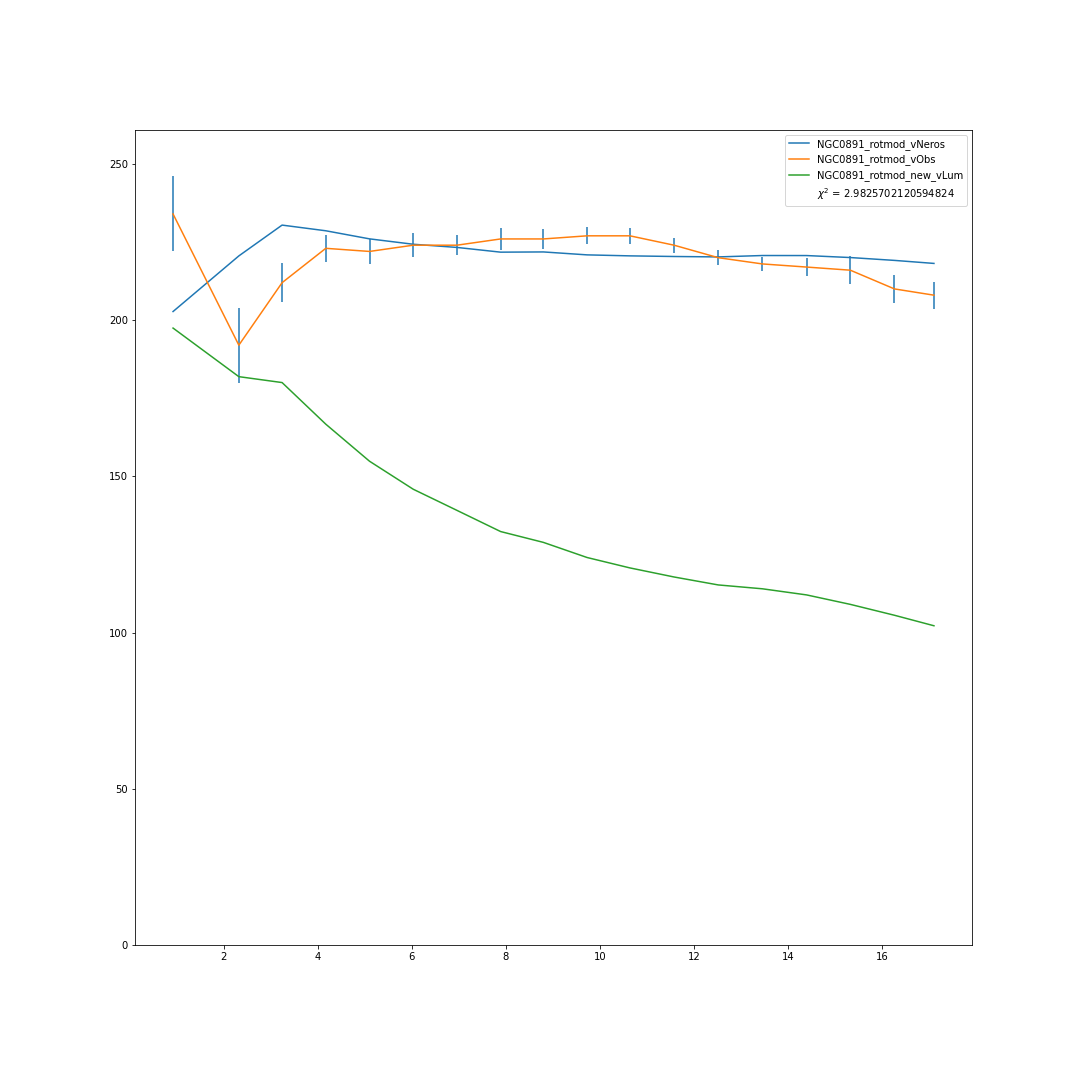
\includegraphics[width=.8\linewidth]{figures/NGC0891_rotmod_XueSofue.png}
  \caption{NGC0891}
  \label{fig:sfig12}
\end{subfigure}
\end{figure}

\clearpage
  \begin{figure}[h]
\begin{subfigure}{.5\textwidth}
  \centering
  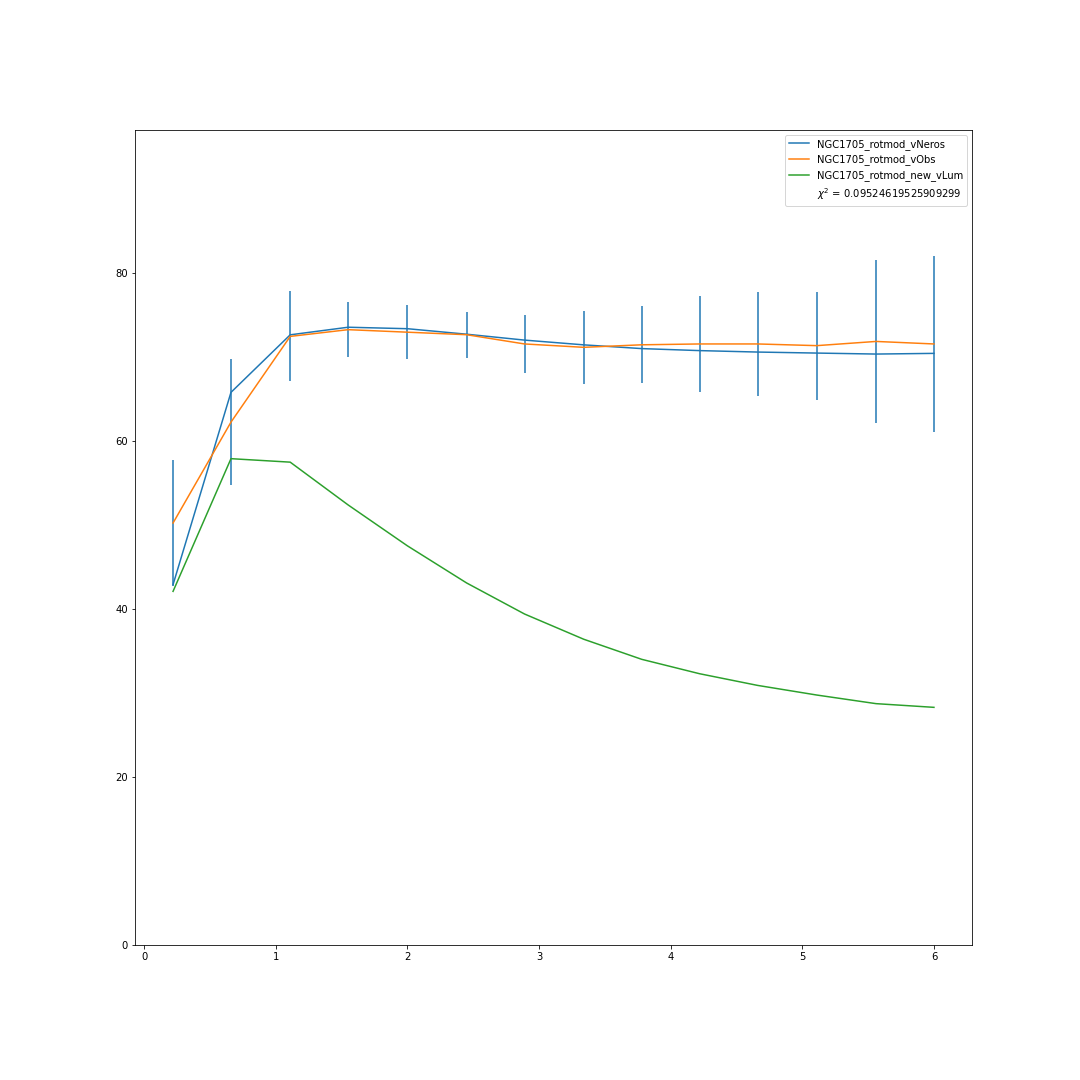
\includegraphics[width=.8\linewidth]{figures/NGC1705_rotmod_XueSofue.png}
  \caption{NGC1705}
  \label{fig:sfig13}
\end{subfigure}
\begin{subfigure}{.5\textwidth}
  \centering
  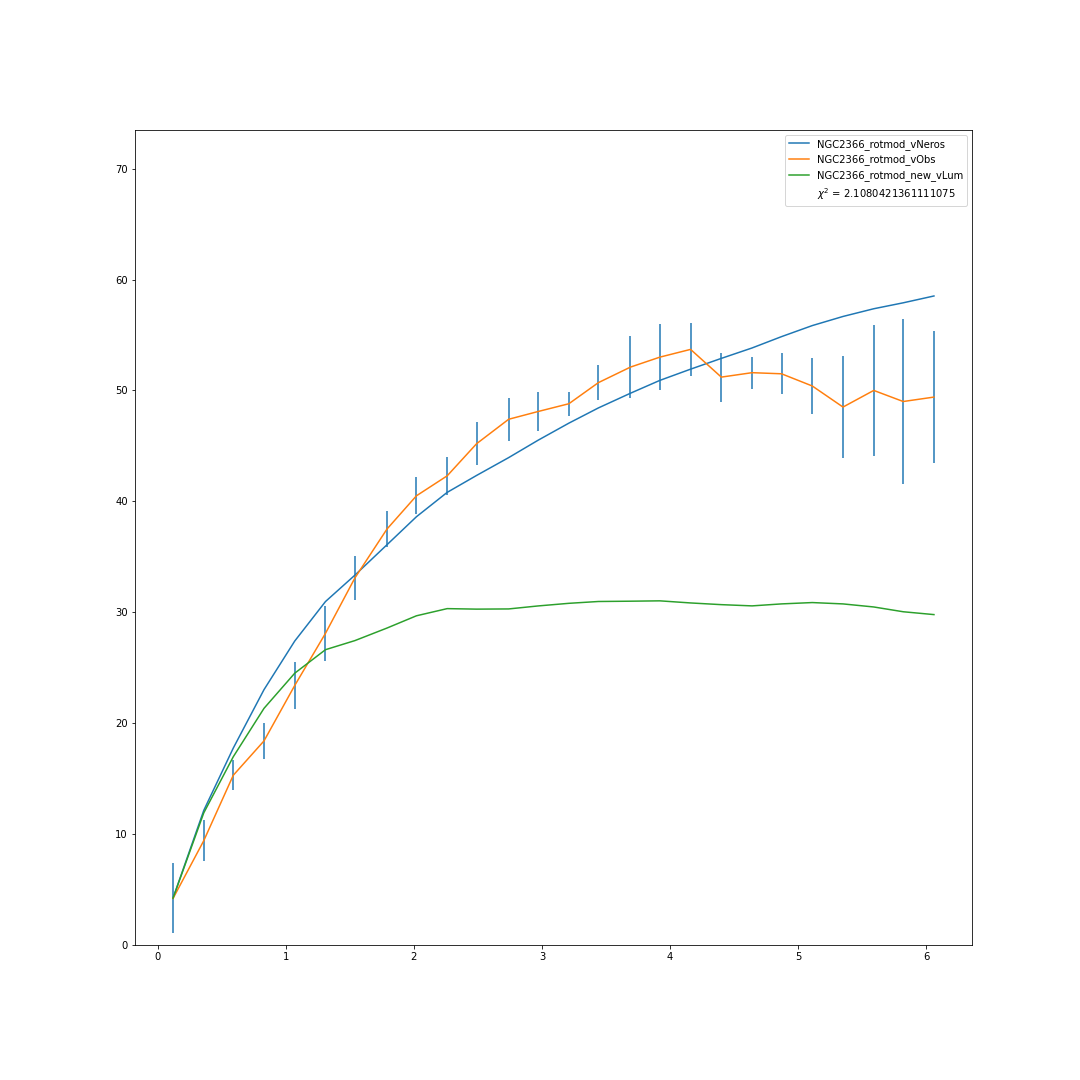
\includegraphics[width=.8\linewidth]{figures/NGC2366_rotmod_XueSofue.png}
  \caption{NGC2366}
  \label{fig:sfig14}
\end{subfigure}%
\begin{subfigure}{.5\textwidth}
  \centering
  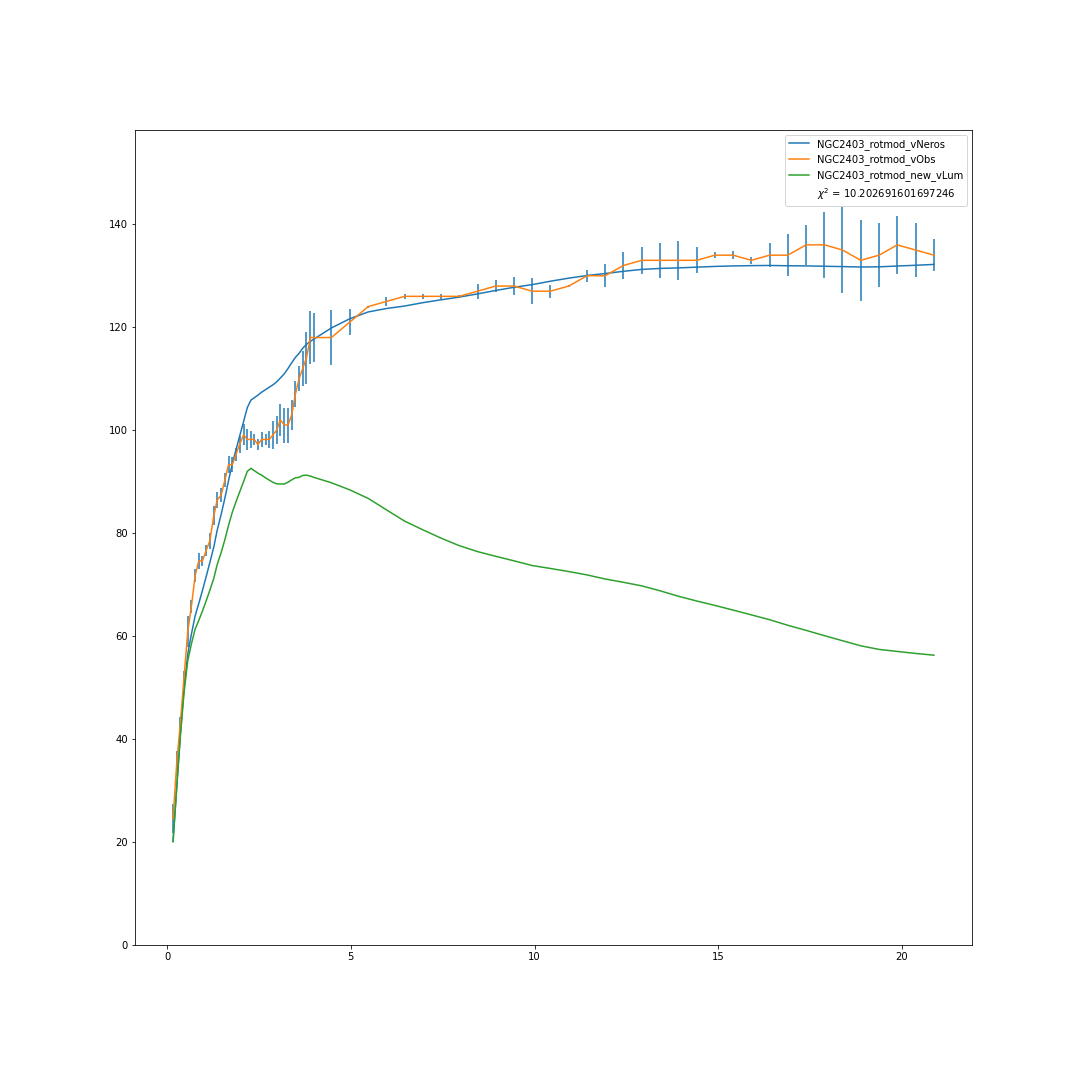
\includegraphics[width=.8\linewidth]{figures/NGC2403_rotmod_XueSofue.png}
  \caption{NGC2403}
  \label{fig:sfig15}
\end{subfigure}
\begin{subfigure}{.5\textwidth}
  \centering
  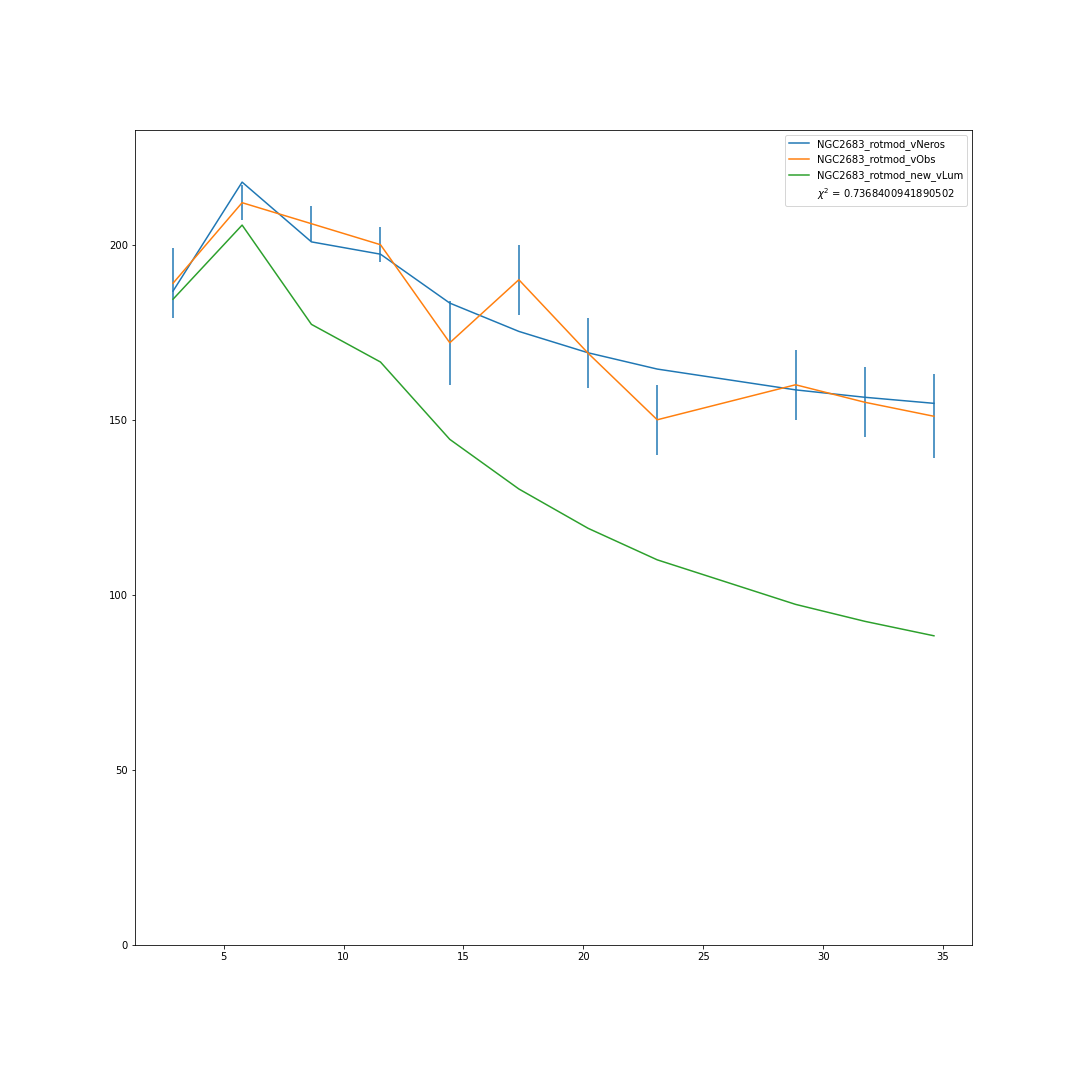
\includegraphics[width=.8\linewidth]{figures/NGC2683_rotmod_XueSofue.png}
  \caption{NGC2683}
  \label{fig:sfig16}
\end{subfigure}
\caption{ }
\label{fig:fig2903}
\end{figure}
%
\clearpage
%
%  
  \begin{figure}[h]
\begin{subfigure}{.5\textwidth}
  \centering
  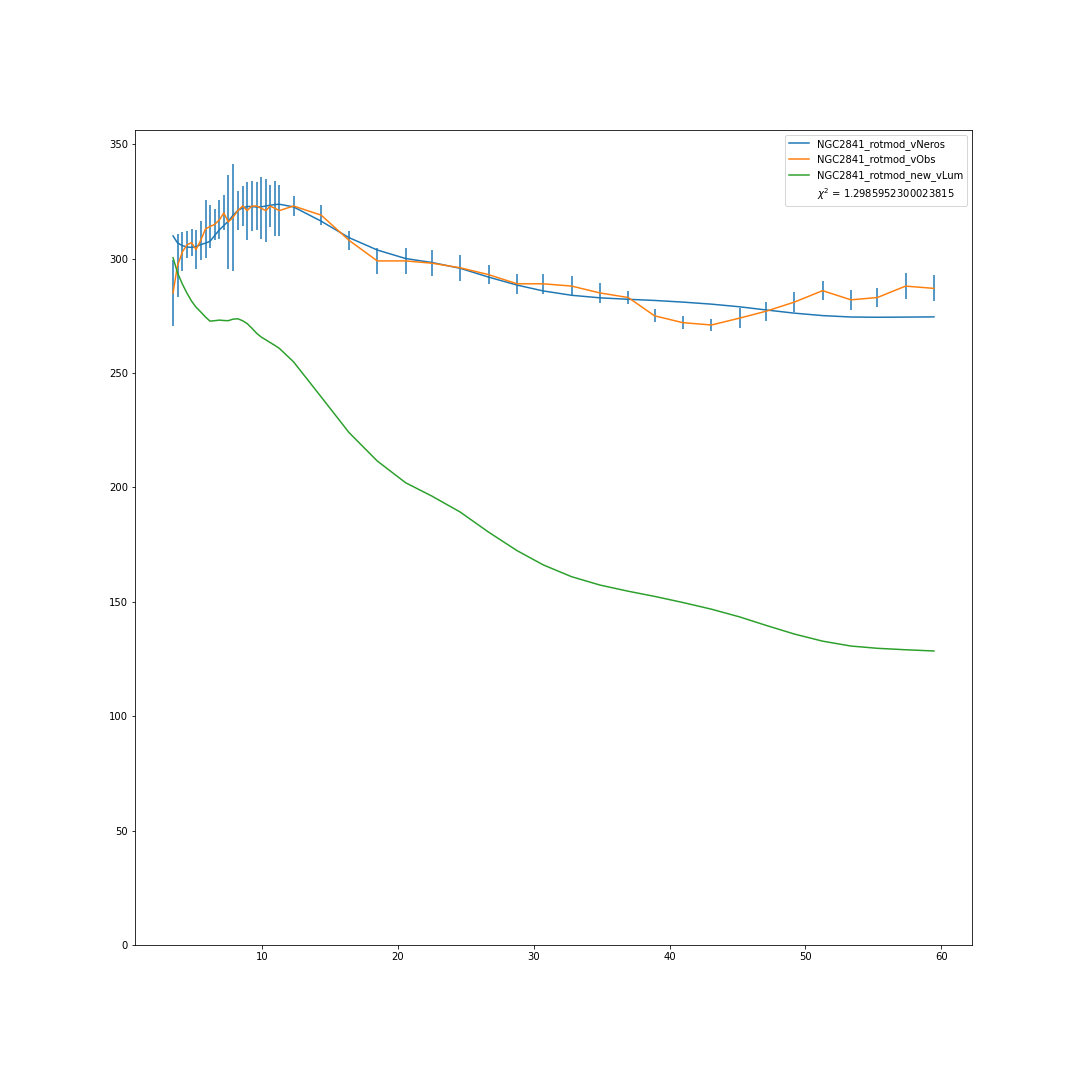
\includegraphics[width=.8\linewidth]{figures/NGC2841_rotmod_XueSofue.png}
  \caption{SPARC\cite{2016Lelli}}
  \label{fig:sfig17}
\end{subfigure}%
\begin{subfigure}{.5\textwidth}
  \centering
  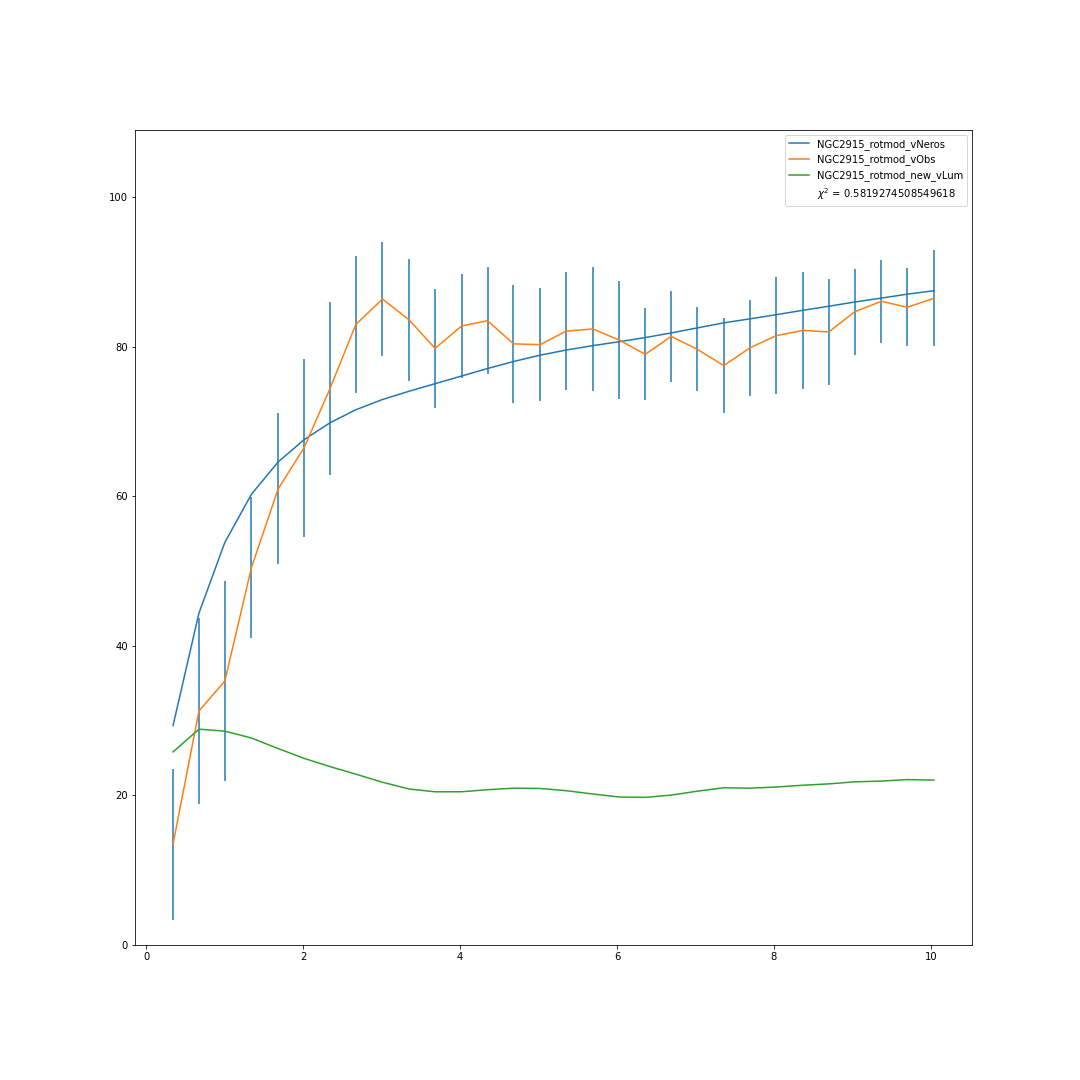
\includegraphics[width=.8\linewidth]{figures/NGC2915_rotmod_XueSofue.png}
  \caption{SPARC\cite{2016Lelli}}
  \label{fig:sfig18}
\end{subfigure}
\caption{ }
\label{fig:fig2915}
\end{figure}
%
%
%
%  
%%%%%%%
  \begin{figure}[h]
\begin{subfigure}{.5\textwidth}
  \centering
  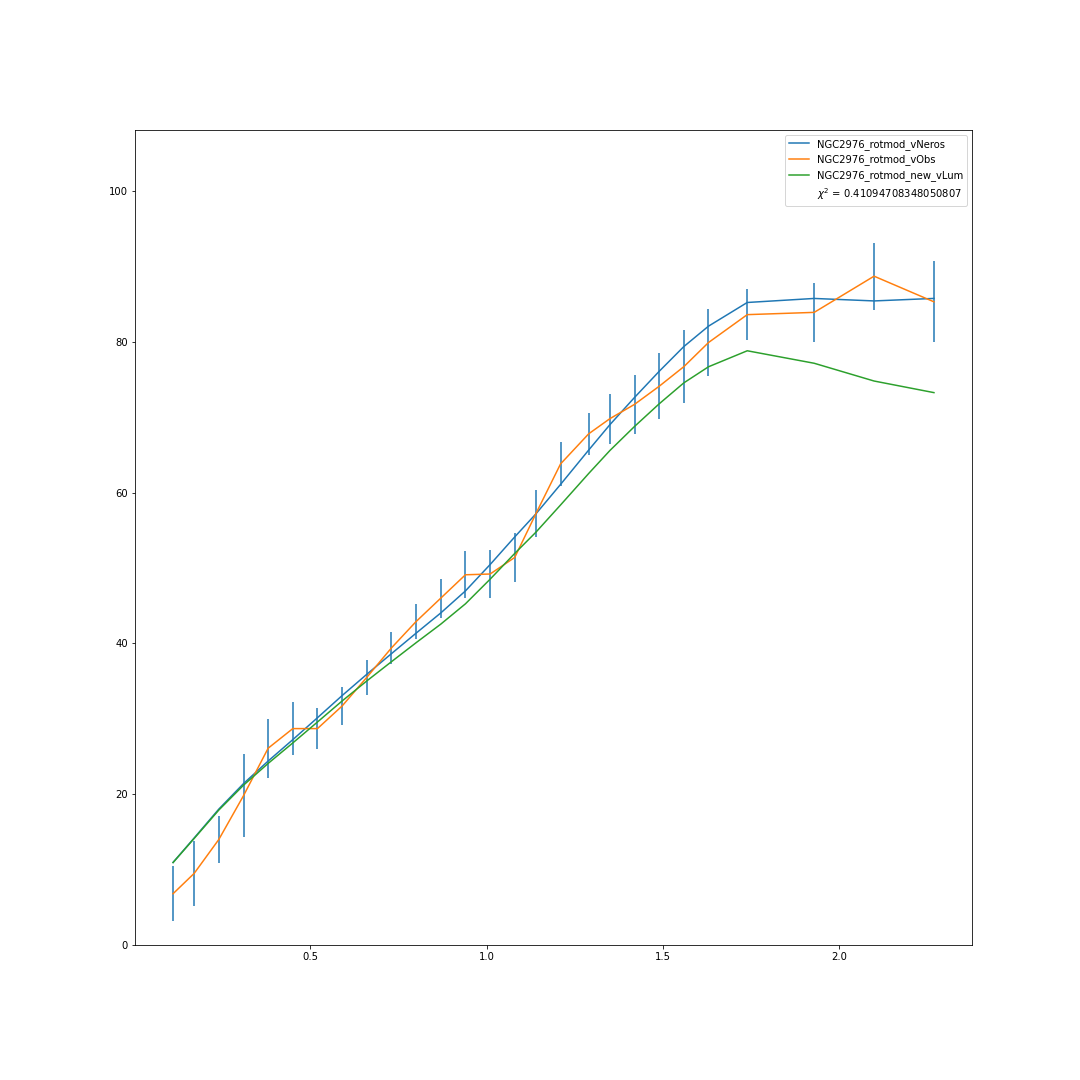
\includegraphics[width=.8\linewidth]{figures/NGC2976_rotmod_XueSofue.png}
  \caption{NGC2976}
  \label{fig:sfig19}
\end{subfigure}%
\begin{subfigure}{.5\textwidth}
  \centering
  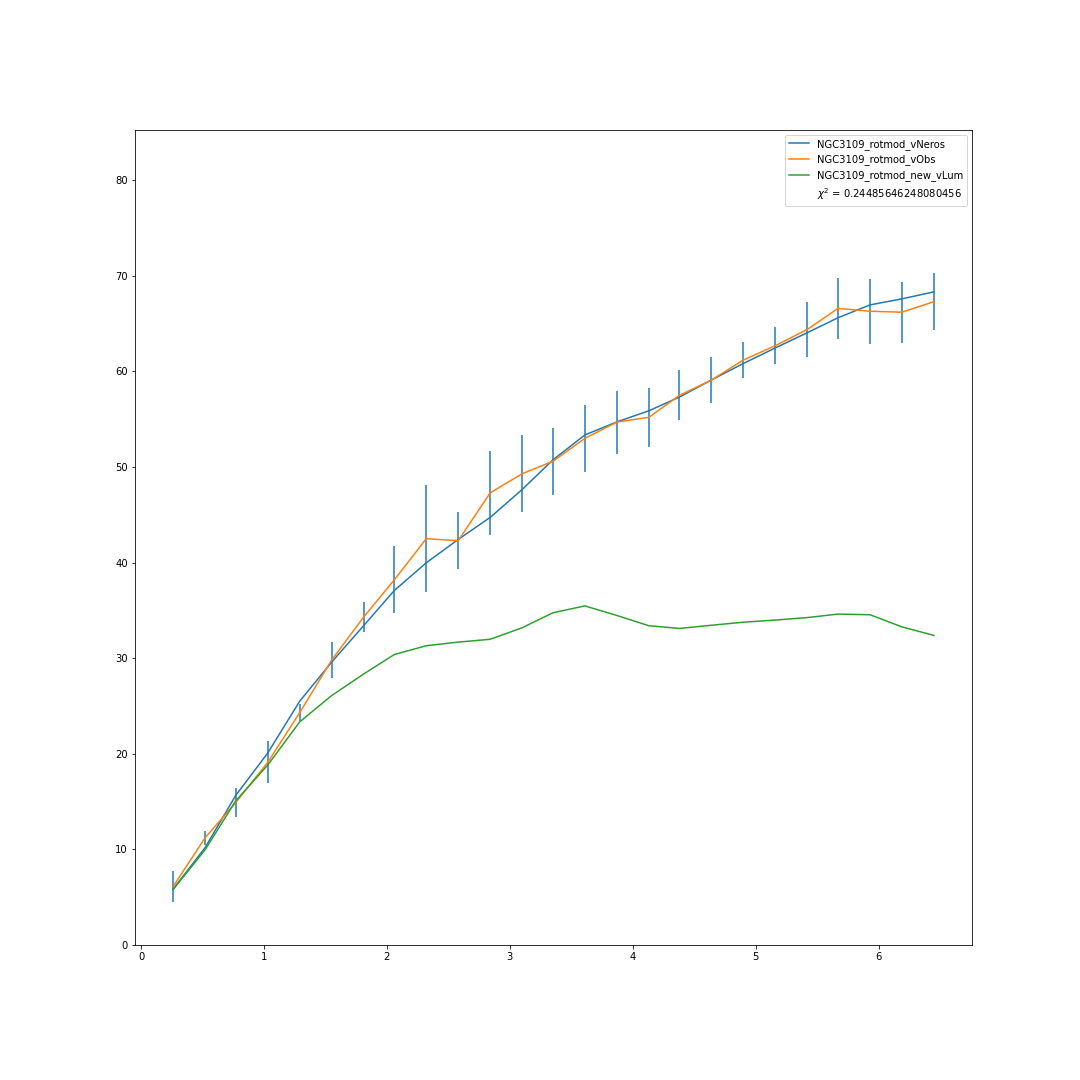
\includegraphics[width=.8\linewidth]{figures/NGC3109_rotmod_XueSofue.png}
  \caption{NGC3109}
  \label{fig:sfig20}
\end{subfigure}
\caption{ }
\label{fig:fig3521}
\end{figure}
%
%
%
\clearpage
 \begin{figure}[h]
\begin{subfigure}{.5\textwidth}
  \centering
  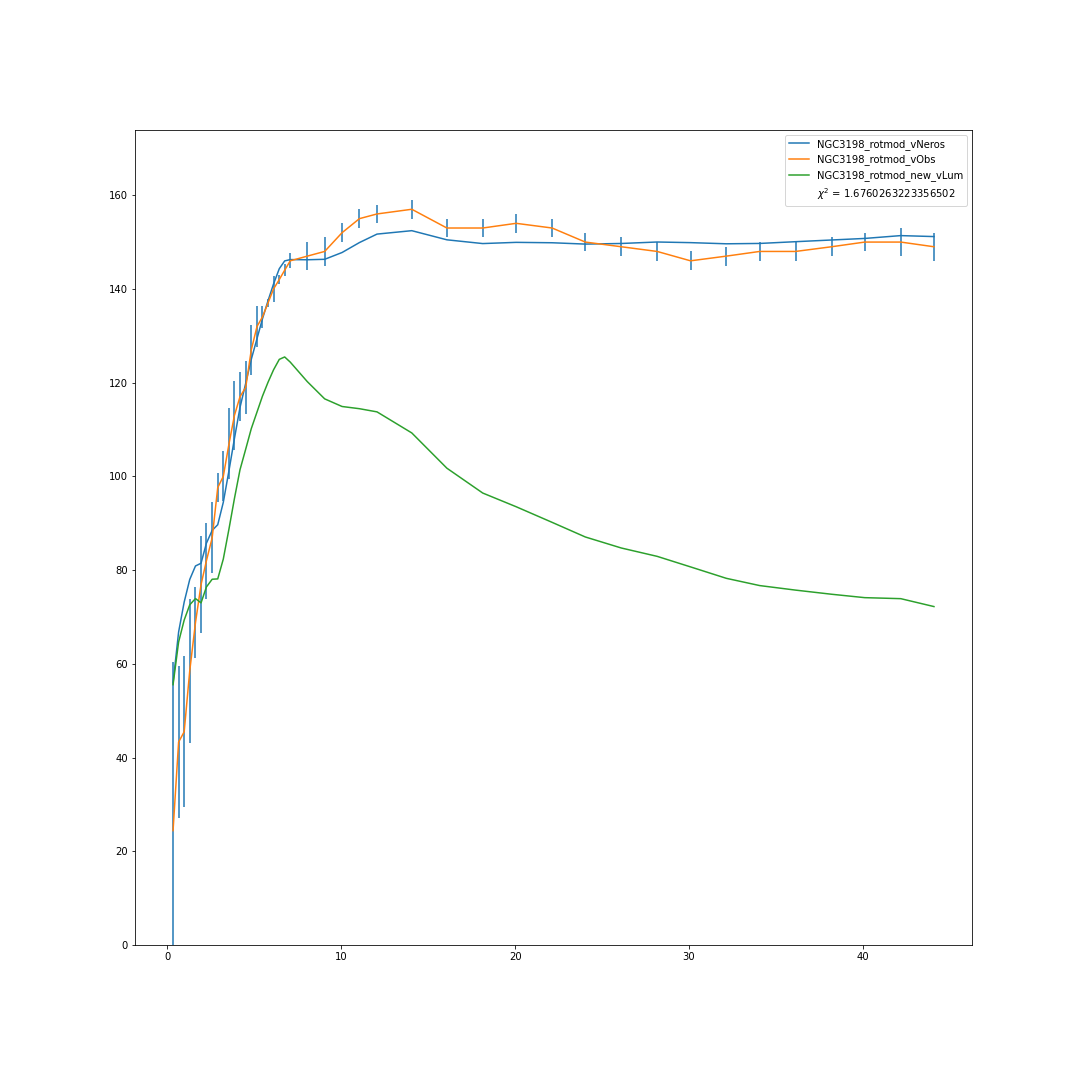
\includegraphics[width=.8\linewidth]{figures/NGC3198_rotmod_XueSofue.png}
  \caption{NGC3198}
  \label{fig:sfig21}
\end{subfigure}%
\caption{ }
\label{fig:fig7331}
\end{figure}
%%%%%%%
 
%%%%%%%%
%%%%%%
%%%%%%%
%%%%%%
  
 

    
     

\bibliography{LCM} 

\end{document}
%
% ****** End of file apssamp.tex ******